\documentclass[a4paper,11pt,twoside,openright,headings=small,numbers=noenddot,parskip=half-]{scrbook}
\PassOptionsToPackage{outputdir=../build/theory}{minted2}
\usepackage{rs3d}
\usepackage[backend=biber,style=authoryear,maxbibnames=6,maxcitenames=2,giveninits=true,uniquename=init,
  sorting=nyt]{biblatex}
\addbibresource{../common/refs.bib}
\graphicspath{{../figures/}}

% ---- notation used throughout (letters only in macro names)
\newcommand{\fs}{f_{\mathrm{s}}}                 % sampling frequency
\newcommand{\fN}{f_{\mathrm{N}}}                 % Nyquist frequency
\newcommand{\dt}{\Delta t}
\newcommand{\df}{\Delta f}
\newcommand{\Tsel}{T_{\mathrm{sel}}}
\newcommand{\abs}[1]{\left|#1\right|}
\newcommand{\E}{\mathbb{E}}
\DeclareMathOperator{\median}{median}
\DeclareMathOperator{\sinc}{sinc}
\newcommand{\jj}{\mathrm{j}}
\newcommand{\dB}{\,\mathrm{dB}}

\hypersetup{pdftitle={RS3D Theory and Algorithms Manual},pdfauthor={RS3D project}}

\begin{document}
\frontmatter
\manualcover{Theory and Algorithms Manual}%
  {The mathematics and signal processing behind every function of the RS3D application}%
  {Edition 1.0 \textbullet\ October 2026 \textbullet\ for rs3d-app 0.1 and later}%
  {Companion to the RS3D User's Guide. All figures are generated by the application's own code from a reproducible synthetic recording.}
\manualheader{Theory and Algorithms Manual}
\chapter*{Preface}
\addcontentsline{toc}{chapter}{Preface}

RS3D is an application for the Raspberry Shake 3D seismograph. Its \emph{User's Guide} explains how to use it;
this manual explains \emph{why it works}. It documents, one function at a time, the signal-processing theory that the
application relies on, how that theory was turned into code, and where the code deliberately or unavoidably departs
from the textbook version.

The manual is written for three kinds of reader: an observer who wants to trust (or question) what a spectrogram or an
alert is telling them, a student who wants a worked example of applied seismological signal processing, and a developer
who is about to change one of the algorithms and needs the assumptions written down.

\paragraph{What is new here, and what is not.}
Nothing in this manual is new science. Every method (Butterworth filtering, Welch spectra, short-time Fourier analysis,
the STA/LTA trigger) is standard and is cited. What the manual adds is precision about \emph{this} implementation:
the exact windows, constants, tolerances and edge-case rules, each traceable to a source file of the application.

\paragraph{How the chapters are organised.}
Chapters follow the path of a sample through the application, from the sensor (Chapters~\ref{ch:data}
and~\ref{ch:response}) through filtering and spectral analysis (Chapters~\ref{ch:filter}--\ref{ch:noise}) and data
quality (Chapter~\ref{ch:quality}) to visualisation, detection and real-time handling
(Chapters~\ref{ch:vis}--\ref{ch:realtime}). Chapter~\ref{ch:arch} describes how the code is organised, and the
appendices collect derivations and every numerical constant used by the application.

\begin{rs3dkey}[How to read the boxes]
\textbf{Key idea} boxes state a result in one or two sentences.\par\smallskip
\textbf{In RS3D} boxes say exactly what the application does, naming the source file (paths are relative to
\file{rs3d-app/src/rs3d/}). Where the application departs from the textbook method this is stated there, never
left implicit.
\end{rs3dkey}

\paragraph{Reproducibility.}
Every plot is produced by one script, \file{make\_figures.py}, which calls the application's own
functions (not re-implementations) on a seeded synthetic recording of one day at a fictitious station
(\file{AM.DEMO1.00}). The recording contains a local earthquake, a distant earthquake, two man-made noise bursts and two
data gaps, so each algorithm can be shown on a case whose true answer is known.

\paragraph{Status of the alert chapter.}
The event-detection theory of Chapter~\ref{ch:detect} is complete. The design of the application's alert pipeline in
Section~\ref{sec:alertdesign} is a \emph{design proposal}: that feature is not yet implemented, and the proposal
will be revised when it is.

\paragraph{Verification of references.}
Two of the key references (Trnkoczy 2012 and McNamara and Buland 2004) were checked against online bibliographic
records while this edition was written. The remaining entries are well-known works cited from the authors'
knowledge; their volume and page numbers should be confirmed against the originals before the references are
reused in a formal publication. The description of rsudp's alert defaults in Chapter~\ref{ch:detect} is deliberately
hedged for the same reason: no authoritative list of defaults could be located.

\bigskip
\begin{center}\small\textsf{\textcolor{rs3dgrey}{RS3D project, October 2026}}\end{center}

\chapter*{Notation}
\addcontentsline{toc}{chapter}{Notation}
\begin{center}
\small
\begin{tabularx}{\linewidth}{@{}l X l@{}}
\toprule
Symbol & Meaning & Unit\\ \midrule
$x(t),\;x[n]$ & continuous signal; its samples $x[n]=x(n\,\dt)$ & counts or m/s\\
$\fs,\;\dt$ & sampling frequency, sampling interval $\dt = 1/\fs$ & Hz, s\\
$\fN$ & Nyquist frequency, $\fN=\fs/2$ & Hz\\
$N$ & number of samples in a window or record & --\\
$T$ & duration $T=N\,\dt$ & s\\
$X[k]$ & discrete Fourier transform of $x[n]$ & counts\\
$f_k$ & frequency of bin $k$, $f_k = k\,\fs/N$ & Hz\\
$\df$ & frequency resolution (bin spacing) $\df=\fs/N=1/T$ & Hz\\
$w[n]$ & window (taper) function & --\\
$H(f)$ & transfer function of a filter & --\\
$T(f)$ & instrument response, counts per unit of ground velocity & counts/(m/s)\\
$S_{xx}(f)$ & one-sided power spectral density & counts$^2$/Hz\\
$\mathrm{STA},\mathrm{LTA}$ & short- and long-term averages & counts$^2$\\
$R$ & STA/LTA ratio & --\\
$\jj$ & imaginary unit & --\\
\bottomrule
\end{tabularx}
\end{center}

\tableofcontents
\mainmatter
\chapter{Introduction}\label{ch:intro}

\section{What the application does}
RS3D reads the three-component ground-velocity signal of a Raspberry Shake 3D, keeps it on the laptop, and turns it
into pictures and numbers an observer can act on. Seen from the signal-processing side its work divides into five
tasks:

\begin{enumerate}
\item \textbf{Acquire}: receive samples in real time (SeedLink) and copy the Shake's day files (SFTP).
\item \textbf{Condition}: convert counts to ground velocity and remove unwanted frequencies.
\item \textbf{Analyse}: estimate spectra, spectrograms and a noise summary; measure data completeness.
\item \textbf{Display}: reduce millions of samples to a few thousand points per plot without losing what matters.
\item \textbf{Detect}: decide, sample by sample, whether the ground is moving more than usual (alerts).
\end{enumerate}

\begin{figure}[tbp]
\centering
\resizebox{\linewidth}{!}{\begin{tikzpicture}[every node/.style={minimum width=2.45cm,minimum height=9mm}]
  \node[boxdark] (shake) at (0,0) {Raspberry Shake 3D\\[-1pt]{\scriptsize 3 geophones, 100 Hz}};
  \node[boxblue] (sl)    at (3.9,1.2)  {SeedLink\\[-1pt]{\scriptsize live, TCP 18000}};
  \node[boxblue] (sftp)  at (3.9,-1.2) {SFTP\\[-1pt]{\scriptsize day files}};
  \node[box]     (ring)  at (6.9,1.2)  {ring buffer\\[-1pt]{\scriptsize 10 minutes}};
  \node[box]     (store) at (6.9,-1.2) {local archive\\[-1pt]{\scriptsize SDS miniSEED}};
  \node[boxblue] (live)  at (9.9,1.2)  {Live view};
  \node[box,dashed] (alert) at (9.9,2.8) {alerts\\[-1pt]{\scriptsize STA/LTA (planned)}};
  \node[box]     (proc)  at (9.9,-1.2) {conditioning\\[-1pt]{\scriptsize units, band-pass}};
  \node[boxblue] (an)    at (12.9,-0.2) {spectrogram\\[-1pt]{\scriptsize noise, health}};
  \node[boxblue] (heli)  at (12.9,-2.2) {helicorder\\[-1pt]{\scriptsize detail, clipboard}};
  \draw[flow] (shake.east) -- ++(0.3,0) |- (sl.west);
  \draw[flow] (shake.east) -- ++(0.3,0) |- (sftp.west);
  \draw[flow] (sl) -- (ring);
  \draw[flow] (sftp) -- (store);
  \draw[flow] (ring) -- (live);
  \draw[flow,dashed] (ring.north) -- ++(0,1.6) -- (alert.west);
  \draw[flow] (store) -- (proc);
  \draw[flow] (proc.east) -- ++(0.35,0) |- (an.west);
  \draw[flow] (proc.east) -- ++(0.35,0) |- (heli.west);
\end{tikzpicture}}
\caption{Data flow of RS3D. Solid boxes exist today; the dashed alert stage is designed in
Section~\ref{sec:alertdesign}.}\label{fig:flow}
\end{figure}

\section{Where each feature is explained}
\Cref{tab:map} links every function a user can see to the chapter that derives it.

\begin{table}[tbp]
\centering\small
\caption{Application features and the chapters that explain them.}\label{tab:map}
\begin{tabularx}{\linewidth}{@{}l X l@{}}
\toprule
Feature & Theory used & Chapter\\ \midrule
Counts / m/s switch & instrument response, deconvolution & \ref{ch:response}\\
Band-pass (Data, Live, Helicorder) & Butterworth, zero-phase filtering & \ref{ch:filter}\\
Spectra mode, clipboard spectrum & discrete Fourier transform, windows & \ref{ch:spectral}\\
Spectrogram & short-time Fourier transform & \ref{ch:spectrogram}\\
Noise spectrum & percentile summary of spectra & \ref{ch:noise}\\
Coverage bar, Data health & gaps, completeness & \ref{ch:quality}\\
Live and helicorder traces, click-to-time & min/max decimation, row geometry & \ref{ch:vis}\\
Alerts & STA/LTA trigger & \ref{ch:detect}\\
Live link, reconnection & SeedLink, buffering, back-off & \ref{ch:realtime}\\
\bottomrule
\end{tabularx}
\end{table}

\section{Conventions}
\paragraph{Time.} All data are stored and processed in UTC. The application can \emph{display} times in the
laptop's local zone, but that only changes labels; no sample is shifted. Times inside the code are epoch seconds
(\code{UTCDateTime.timestamp}).

\paragraph{Amplitude units.} Unless stated otherwise amplitudes are in \emph{counts}, the integers produced by the
Shake's analogue-to-digital converter. Chapter~\ref{ch:response} explains the conversion to ground velocity in m/s.

\paragraph{Decibels.} A power ratio of $P$ is $10\log_{10}P$~dB; an amplitude ratio of $A$ is $20\log_{10}A$~dB. The
application's spectrograms use $10\log_{10}$ of power spectral density in counts$^2$/Hz, written
``dB re.\ 1~count$^2$/Hz''.

\begin{rs3dnote}[Software versions]
The application was developed against ObsPy~1.5.1 \parencite{beyreuther2010,krischer2015}, SciPy~1.x and
NumPy. Where behaviour depends on a library default (for example SciPy's spectrogram window or ObsPy's response
removal), the default is stated and was checked directly against the installed library.
\end{rs3dnote}

\chapter{Seismic data fundamentals}\label{ch:data}

\section{From ground motion to numbers}
A seismometer converts ground motion into an electrical signal. The Raspberry Shake 3D carries three orthogonal
geophones, nominally with a natural frequency of $f_0 = 4.5$~Hz, one vertical (Z) and two horizontal (N--S and E--W).
A geophone is a coil suspended in the field of a magnet fixed to the case. When the ground, and with it the case,
moves, the coil lags behind by inertia, and the relative velocity between coil and magnet induces a voltage
proportional to that \emph{relative velocity}. Above its natural frequency the relative velocity of the coil equals
the ground velocity, so the voltage is proportional to ground velocity in the pass band
(Chapter~\ref{ch:response} derives the transfer function; \textcite{havskov2016} treat the physics in depth).

The analogue voltage is then amplified and digitised by an analogue-to-digital converter (ADC). The integers it
produces are called \emph{counts}. A count is not a physical unit: one count corresponds to a fixed number of
volts, and, through the sensor, to a frequency-dependent velocity. The conversion is the subject of
Chapter~\ref{ch:response}.

\section{Sampling and the Nyquist frequency}
The ADC measures the signal at regular intervals $\dt$, giving samples $x[n]=x(n\,\dt)$. The Raspberry Shake 3D
samples at $\fs = 100$~samples per second, so $\dt = 10$~ms. The sampling theorem states that a band-limited signal
can be reconstructed exactly from its samples if and only if it contains no energy at or above the
\emph{Nyquist frequency}
\begin{equation}
  \fN = \frac{\fs}{2} = 50\ \text{Hz}.
\end{equation}
Energy above $\fN$ does not vanish when sampled: it \emph{aliases}, folding back into the band below $\fN$. A
sinusoid of frequency $f$ with $\fN < f < \fs$ produces exactly the same samples as one of frequency $\fs - f$
(\cref{fig:alias}). Aliasing cannot be undone after sampling, so digitisers apply an analogue and digital
\emph{anti-alias filter} before and during decimation; its roll-off is visible as a fall in the spectra of RS3D
near $\fN$ (Chapter~\ref{ch:noise}). Consequently the top few hertz of any RS3D spectrum are attenuated by the
instrument, not by the ground.

\begin{figure}[tbp]
\centering
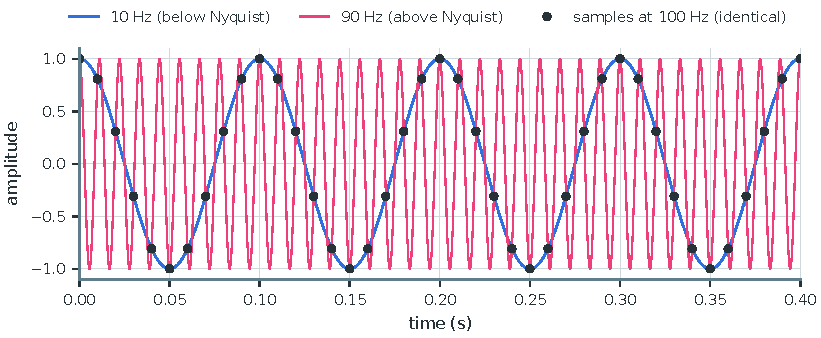
\includegraphics[width=\linewidth]{theory-aliasing}
\caption{Aliasing. At $\fs = 100$~Hz a 90~Hz cosine (pink) and a 10~Hz cosine (blue) have identical samples
(dots). Because $90 = \fs - 10$, the faster signal is indistinguishable from the slower one after sampling.}\label{fig:alias}
\end{figure}

\begin{rs3dkey}
Everything the application shows lies below $\fN = 50$~Hz, and the last few hertz below it are shaped by the
Shake's anti-alias filter.
\end{rs3dkey}

\section{Channel naming}
Every stream of samples is identified by four codes, the SEED identifier \parencite{fdsnseed2012}:
\begin{center}\ttfamily\small
\begin{tabular}{@{}llll@{}}
\textcolor{rs3dgrey}{network} & \textcolor{rs3dgrey}{station} & \textcolor{rs3dgrey}{location} & \textcolor{rs3dgrey}{channel}\\
AM & R77A7 & 00 & EHZ
\end{tabular}
\end{center}
\code{AM} is the Raspberry Shake network, \code{R77A7} the station, \code{00} the location code. The three-letter
channel code is itself structured: \code{E} is the \emph{band} code (an extremely short-period instrument sampled at
80~Hz or more), \code{H} the \emph{instrument} code (a high-gain seismometer), and the last letter the
\emph{orientation}: \code{Z} vertical, \code{N} north--south, \code{E} east--west. An RS3D therefore serves
\code{EHZ}, \code{EHN} and \code{EHE}. The application sorts channels vertical-first (\code{Z}, \code{N}, \code{E})
so that the default channel is always the vertical.

\section{miniSEED and the day archive}
Seismic samples are exchanged as \emph{miniSEED}, a sequence of fixed-length records (512 bytes is typical for
SeedLink). Each record carries the four identifier codes, the time of its first sample, the sampling rate, and a block
of samples stored as first differences compressed with the Steim algorithm. Because consecutive samples of a smooth
signal differ by small amounts, the compression is lossless and efficient. One channel-day is 8.64~million samples,
about 35~MB as raw 32-bit integers; the Shake's compressed archive for all three channels takes about 85~MB per
day (the figure quoted in the application's own storage help).

A \emph{gap} is a place where a record's start time does not continue the previous record. Readers such as ObsPy
split a stream at gaps into separate \emph{traces}; the application keeps them separate (and shows them as breaks
or blank columns) rather than inventing data. How gaps are measured is the subject of Chapter~\ref{ch:quality}.

Files are arranged in the \emph{SeisComP data structure} (SDS), one file per channel per day:
\begin{center}
\code{<root>/YEAR/NET/STA/CHAN.D/NET.STA.LOC.CHAN.D.YEAR.DOY}
\end{center}
where \code{DOY} is the day of the year, zero-padded to three digits. For example the vertical channel of
15~October 2026 is stored in \file{2026/AM/R77A7/EHZ.D/AM.R77A7.00.EHZ.D.2026.288}. The Shake keeps the same layout
under \file{/opt/data/archive}, and the application mirrors it on the laptop, so a file downloaded from the Shake
can be used unchanged.

\begin{rs3dapp}
\file{core/store.py} implements the day-file layout (\code{day\_path}, \code{days}, \code{load}); \code{import\_file}
splits any miniSEED file into day files, merging with data already present so that importing the same file twice
changes nothing. \file{core/archive.py} copies day files from the Shake: it downloads into a temporary \file{.part}
file and renames it only when complete, so an interrupted transfer never looks like a finished day, and it
always re-fetches the newest remote day because the Shake is still writing to it.
\end{rs3dapp}

\section{Time}
Sample times are UTC. The time of sample $n$ of a record starting at $t_0$ is $t_0 + n/\fs$. The accuracy of
$t_0$ depends entirely on the Shake's clock, which is kept right by the network time protocol; an offset of
100~ms is already visible when two stations are compared. The Status page therefore flags a clock offset above
100~ms as a warning and above 1000~ms as an error (\file{core/status.py}). Leap seconds are not modelled:
timestamps are POSIX-style seconds, which is adequate for the minute-to-second resolution the application targets.

\chapter{Instrument response and units}\label{ch:response}

\section{Why counts are not ground motion}
A record in counts mixes two things: the ground motion and the way the instrument responds to it. The same ground
velocity at 0.1~Hz and at 10~Hz produces very different counts, because a geophone responds weakly below its natural
frequency. To compare records from different instruments, or to report ground velocity, the instrument's effect must
be removed. This is done with the \emph{instrument response}.

\section{Linear systems and the transfer function}
Over its operating range a seismometer behaves as a linear, time-invariant system. If the ground velocity is
$v(t)$ and the digitised output is $d(t)$ (in counts), then in the frequency domain
\begin{equation}
  D(f) = T(f)\,V(f),
\end{equation}
where $V$ and $D$ are the Fourier transforms of $v$ and $d$ and $T(f)$ is the complex \emph{transfer function}, in
counts per (m/s). Its magnitude $\abs{T}$ says how much each frequency is amplified; its phase says how much it is
delayed.

\subsection{A geophone as a second-order system}
The mechanical part of a geophone is a damped oscillator. With natural angular frequency
$\omega_0 = 2\pi f_0$ and fractional damping $h$ the velocity transfer function in the Laplace variable
$s=\jj\omega$ is
\begin{equation}\label{eq:geophone}
  T_g(s) = G\,\frac{s^{2}}{s^{2} + 2h\,\omega_0\,s + \omega_0^{2}},
\end{equation}
where $G$ is the generator constant (volts per m/s) in the flat band. Equation~\eqref{eq:geophone} has two zeros at
$s=0$ and two poles at $s=\omega_0\bigl(-h \pm \jj\sqrt{1-h^2}\bigr)$. \Cref{fig:response} shows its magnitude and
phase for $f_0 = 4.5$~Hz.

\begin{figure}[tbp]
\centering
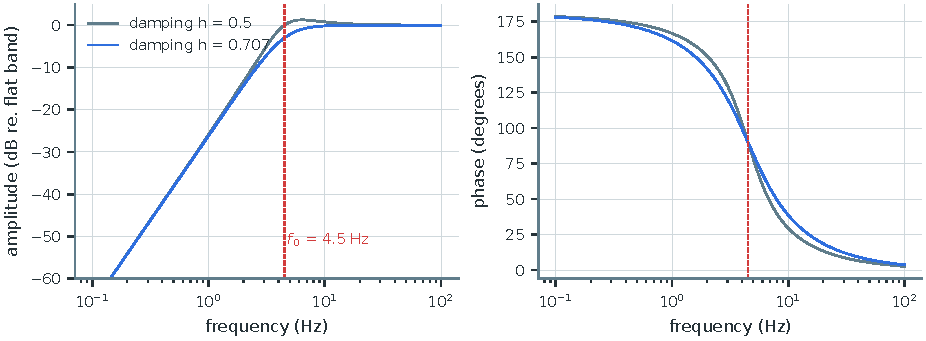
\includegraphics[width=\linewidth]{theory-response}
\caption{Magnitude and phase of the velocity response~\eqref{eq:geophone} of a 4.5~Hz geophone for two damping
values. Illustrative only: the real response of a given Shake comes from its StationXML file.}\label{fig:response}
\end{figure}

Three properties matter for what follows.
\begin{enumerate}
\item \textbf{Flat above $f_0$.} For $f\gg f_0$, $T_g\to G$: the output follows ground velocity directly.
\item \textbf{Falling as $f^{2}$ below $f_0$.} The double zero at the origin makes the response fall at 40~dB per
  decade (a factor 100 in amplitude for each factor 10 in frequency).
\item \textbf{Zero at $f=0$.} A constant (DC) input produces no output from the mechanical part.
\end{enumerate}

\subsection{The complete chain}
The digitiser adds its own stages: amplification, a digital anti-alias filter and decimation. The \emph{overall}
response is the product of the stage responses. Standards describe it as poles, zeros and a normalisation, and
distribute it as \emph{StationXML}. In the flat band the overall response reduces to a single number, the
\emph{sensitivity} $\Lambda$ in counts per m/s.

\section{Removing the response}
Estimating the ground velocity means dividing by $T$ in the frequency domain:
\begin{equation}\label{eq:deconv}
  \hat v(t) = \mathcal{F}^{-1}\!\left[\frac{D(f)}{T(f)}\right].
\end{equation}
Equation~\eqref{eq:deconv} hides a numerical trap. Below $f_0$, $\abs{T}$ becomes very small, so dividing by it
\emph{amplifies} whatever is there, which is mostly noise, and at $f=0$ the division is by zero. Practical
implementations therefore (i) remove the mean first, (ii) taper the record so that its ends do not create
discontinuities, and (iii) limit the division with a \emph{water level}: wherever $\abs{T}$ falls below a chosen
fraction of its maximum, it is replaced by that fraction.

\begin{rs3dapp}
The \ui{counts}/\ui{m/s} switch calls ObsPy's \code{remove\_response(inventory, output="VEL")} in
\file{core/export.py}, with ObsPy's defaults, which were read from the installed library: zero-mean removal on, a
5\,\% cosine taper, a water level of 60~dB, and no pre-filter. The response is a StationXML file downloaded once from
the Raspberry Shake FDSN web service and cached in the data folder (\file{core/response.py}); with the file cached
the switch works offline. Without a cached response and without Internet the Data page reports the error, and the Helicorder page
reports it and returns to counts instead of showing an empty chart.
\end{rs3dapp}

\begin{rs3dwarn}[Velocity below the natural frequency]
Because the response is deconvolved with a water level, ground velocity at frequencies well below
4.5~Hz is only as reliable as the signal-to-noise ratio there. Long-period phenomena, such as the ocean microseism near
0.2~Hz or the surface waves of distant earthquakes, are recoverable but noisier than the same signal on a broadband
sensor.
\end{rs3dwarn}

\section{The DC offset}
Raw counts almost never oscillate around zero. Electronic offsets in the sensor and ADC add a constant,
typically thousands of counts for a Shake. Because $T(0)=0$, such a constant is \emph{not} ground motion, and any
processing that does not remove it has to cope with it:

\begin{itemize}
\item \textbf{Spectra.} An offset leaks into the lowest bins and, through window sidelobes, into higher ones.
  The application subtracts the mean before every spectrum (Chapter~\ref{ch:spectral}).
\item \textbf{Filtering.} The filter route removes the mean before filtering (\code{detrend("demean")} in
  \file{core/export.py}).
\item \textbf{The helicorder.} Plotting raw counts would shift every row by the offset and dominate the amplitude
  scale (\cref{fig:dcoffset} in Chapter~\ref{ch:vis}); each row therefore has its median removed.
\end{itemize}

\begin{rs3dkey}
Counts are an instrument-dependent integer with an arbitrary offset. Ground velocity needs the response; every
display that does not use it must at least remove the mean.
\end{rs3dkey}

\chapter{Digital filtering}\label{ch:filter}

A filter keeps some frequencies and suppresses others. The application offers a band-pass filter on the Data,
Live and Helicorder pages: slow drifts below the lower corner and electrical or traffic noise above the upper
corner are removed, leaving the band in which the phenomenon of interest lives.

\section{Frequency response of a digital filter}
A linear filter acts on a sampled signal by convolution, $y[n]=\sum_m h[m]\,x[n-m]$. Its effect at frequency $f$ is
described by $H(f)=\sum_m h[m]\,e^{-\jj 2\pi f m/\fs}$, a complex number whose magnitude is the \emph{gain} and whose
angle is the \emph{phase shift}. A band-pass filter has gain close to 1 between two \emph{corner frequencies}
$f_1<f_2$ and gain close to 0 outside.

\section{The Butterworth filter}
Among the classical filter families, the Butterworth filter \parencite{butterworth1930} has the property that its
magnitude is as flat as possible in the pass band. The magnitude of a Butterworth low-pass filter of order $n$ and
cut-off $\omega_c$ is
\begin{equation}\label{eq:butter}
  \abs{H(\jj\omega)}^{2} = \frac{1}{1+\left(\omega/\omega_c\right)^{2n}} .
\end{equation}
At $\omega=\omega_c$ the gain is $1/\sqrt2$, that is $-3$~dB, for every order. Beyond the cut-off the gain falls by
$20n$~dB per decade ($6n$~dB per octave), so a higher order gives a steeper edge. A band-pass filter is obtained from a
low-pass prototype by the substitution $s\mapsto (s^{2}+\omega_1\omega_2)/\bigl(s(\omega_2-\omega_1)\bigr)$, which
doubles the number of poles: an order-$n$ band-pass has $2n$ poles. Digital implementations realise the filter as a
cascade of second-order sections (SOS) rather than one high-order polynomial, because the cascade is numerically
far more stable.

\begin{figure}[tbp]
\centering
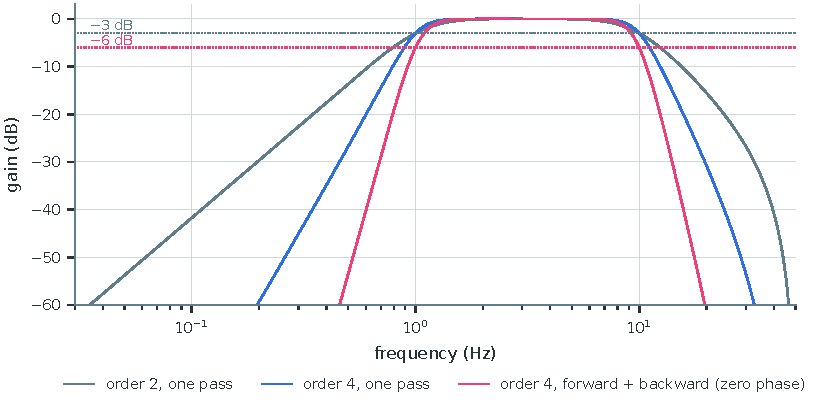
\includegraphics[width=\linewidth]{theory-butterworth}
\caption{Gain of band-pass Butterworth filters with corners 1 and 10~Hz at $\fs=100$~Hz: order~2 and order~4 in a
single pass, and order~4 applied forward and backward (zero phase), whose gain in decibels is exactly twice that of
one pass.}\label{fig:butter}
\end{figure}

\section{Zero-phase filtering}
A causal filter delays different frequencies by different amounts (phase distortion), which smears and shifts
waveforms. A standard remedy is to filter the record forward, reverse the output, filter it again, and reverse the
result. If one pass has frequency response $H(f)$, the backward pass contributes $H^{*}(f)$ (the complex conjugate),
so the combined response is
\begin{equation}\label{eq:zerophase}
  H_{\mathrm{zp}}(f) = H(f)\,H^{*}(f) = \abs{H(f)}^{2},
\end{equation}
a real, non-negative number: \emph{zero phase shift}. Two consequences follow from~\eqref{eq:zerophase}:

\begin{enumerate}
\item \textbf{The gain in decibels doubles.} The $-3$~dB corner of a single pass becomes a $-6$~dB corner
  (\cref{fig:butter}), and the roll-off steepens to $12n$~dB per octave.
\item \textbf{The filter is non-causal.} The output at time $t$ depends on input after $t$.
\end{enumerate}

\begin{rs3dwarn}[Non-causal filters move energy before the onset]
A zero-phase filter smears the sharp start of an arrival \emph{backwards} in time, as \cref{fig:zerophase} shows: the
filtered record contains oscillations before the true onset. Zero-phase filtering is therefore appropriate for
looking at a waveform, but it must not be used to pick onset times or to drive a real-time trigger. The detector of
Chapter~\ref{ch:detect} uses a causal filter for exactly this reason.
\end{rs3dwarn}

\begin{figure}[tbp]
\centering
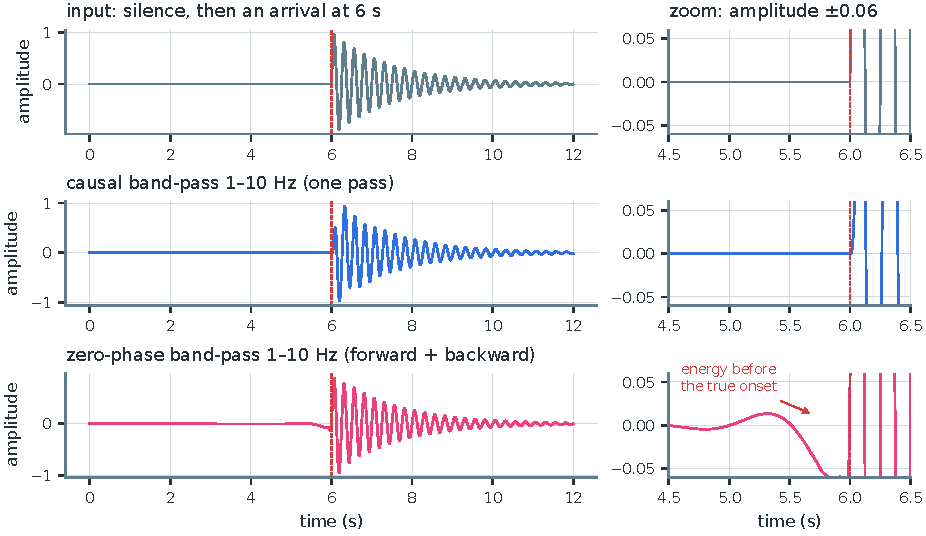
\includegraphics[width=\linewidth]{theory-zerophase}
\caption{An ideal arrival at 6~s filtered by a 1--10~Hz band-pass, causally (one pass) and with zero phase. The
causal output is exactly zero before the arrival; the zero-phase output rings before it (enlarged on the right).
The zero-phase curve was computed with SciPy's padded \code{sosfiltfilt}.}\label{fig:zerophase}
\end{figure}

\section{Edge effects}
A filter has a memory: its output near the start of a record depends on samples that were never recorded. The first
and last seconds of a filtered trace contain a \emph{transient} and are less reliable. The effect is largest for narrow
bands and low corners; a practical rule is to distrust about $3/f_1$ seconds at each end. The same holds at
every \emph{gap}: each contiguous piece of a trace is filtered on its own, so the edges of each piece carry a
transient.

\section{Choosing a band}
\Cref{tab:bands} lists bands commonly used with a short-period sensor such as the RS3D. They are starting points, not
rules; the right band depends on the noise at the site (Chapter~\ref{ch:noise}).

\begin{table}[tbp]
\centering\small
\caption{Typical pass bands for three-component short-period data.}\label{tab:bands}
\begin{tabularx}{\linewidth}{@{}l c X@{}}
\toprule
Purpose & Band (Hz) & Comment\\ \midrule
Local and regional earthquakes & 1--10 & the RS3D live default; rejects drift and most wind or traffic noise\\
Teleseismic body waves & 0.5--3 & the Shake's sensitivity falls quickly below its 4.5~Hz natural frequency\\
Microseism & 0.1--0.5 & strong everywhere; useful as a check of the instrument\\
Cultural noise & 5--25 & footsteps, traffic, machinery\\
\bottomrule
\end{tabularx}
\end{table}

\begin{rs3dapp}
RS3D uses two different implementations, deliberately.
\begin{itemize}
\item \textbf{Data and Helicorder pages, exports} (\file{core/export.py}). ObsPy's
  \code{filter("bandpass", freqmin, freqmax, corners=4, zerophase=True)} after \code{detrend("demean")}.
  Reading the library source and comparing outputs shows that ObsPy implements \code{zerophase} as two passes of an
  SOS filter (forward, then backward) \emph{without} padding, so edge transients are visible; the result is identical
  to two calls of \code{sosfilt}. Corner~4 means a 4th-order design, so the effective roll-off is 48~dB per octave per
  edge.
\item \textbf{Live page} (\file{core/live.py}). SciPy's \code{butter(2, [f\_min, min(f\_max, 0.45 fs)])} applied with the
  padded \code{sosfiltfilt} to each contiguous chunk of the ring buffer, after removing the chunk's mean. The upper
  corner is limited to $0.45\,\fs=45$~Hz to stay below the Nyquist frequency, and a chunk shorter than the padding
  length is only demeaned and not filtered.
\end{itemize}
Both give a zero-phase band-pass; they differ in order and in edge treatment. The numbers a filtered Live trace shows
therefore differ slightly from the same interval exported from the Data page.
\end{rs3dapp}

\section{Summary}
\begin{rs3dkey}
A Butterworth band-pass applied forward and backward is a zero-phase filter whose corner gain is $-6$~dB, whose
roll-off is twice that of one pass, and which is \emph{not} causal. Use it to look at waveforms; use a causal filter
to detect them.
\end{rs3dkey}

\chapter{Spectral analysis}\label{ch:spectral}

The \ui{Spectra} mode of the Helicorder detail view and the third panel of the Waveform Clipboard show an
\emph{amplitude spectrum}: how large the oscillation is at each frequency in a window of data. This chapter derives
what that number means and how the application computes it.

\section{The discrete Fourier transform}
For $N$ samples $x[0],\dots,x[N-1]$ the discrete Fourier transform (DFT) is
\begin{equation}\label{eq:dft}
  X[k] = \sum_{n=0}^{N-1} x[n]\,e^{-\jj 2\pi k n/N}, \qquad k=0,\dots,N-1.
\end{equation}
Bin $k$ corresponds to frequency $f_k = k\,\fs/N$. For real data the bins above $k=N/2$ mirror those below, so only
$k=0,\dots,N/2$ (frequencies from 0 to $\fN$) are kept; this is the \emph{one-sided} spectrum. The spacing of the bins,
\begin{equation}\label{eq:resolution}
  \df = \frac{\fs}{N} = \frac{1}{T},
\end{equation}
is the \emph{frequency resolution}: observing for $T$ seconds cannot separate two frequencies closer than $1/T$.
The practical meaning is stated by the rule \emph{longer observation, finer spectrum}.

\section{Windowing and spectral leakage}
Computing a DFT of a finite record is the same as multiplying an infinitely long signal by a rectangular window
of length $N$. Multiplication in time is convolution in frequency, so the spectrum of the signal is convolved with
the spectrum of the window: a narrow \emph{main lobe} and a series of \emph{sidelobes}. A pure tone that does not
fall exactly on a bin is smeared into neighbouring bins, and the sidelobes of a strong tone can bury a weak one. This
is \emph{spectral leakage}.

A \emph{taper} that smoothly reduces the data to zero at both ends lowers the sidelobes, at the price of a wider
main lobe. The Hann window
\begin{equation}\label{eq:hann}
  w[n] = \tfrac12\Bigl(1-\cos\frac{2\pi n}{N-1}\Bigr),\qquad n=0,\dots,N-1,
\end{equation}
is the common compromise \parencite{harris1978}. \Cref{fig:leak} shows a strong tone at 5.05~Hz and a tone 50~dB
weaker at 8~Hz: with the rectangular window the weak tone is invisible in the leakage, with the Hann window it is
clearly separated.

\begin{figure}[tbp]
\centering
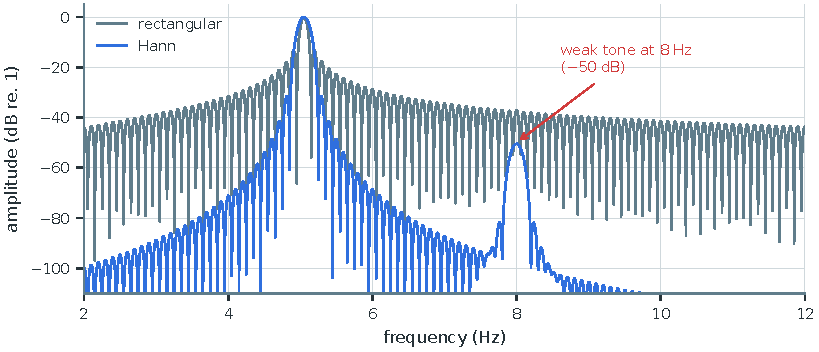
\includegraphics[width=\linewidth]{theory-window-leakage}
\caption{Leakage. Spectrum of a tone at 5.05~Hz (not on a bin) plus a tone 50~dB weaker at 8~Hz, $N=1000$ samples at
100~Hz. The Hann window (blue) reveals the weak tone that the rectangular window (grey) hides.}\label{fig:leak}
\end{figure}

\Cref{tab:windows} gives the measured properties of the three windows used by the application. They were computed
numerically for $N=1024$ with a zero-padded transform.

\begin{table}[tbp]
\centering\small
\caption{Properties of the windows used in RS3D. $\sum w/N$ is the coherent gain; ENBW (equivalent noise bandwidth)
and the null-to-null main-lobe width are in bins; the peak sidelobe is relative to the peak.}\label{tab:windows}
\setlength{\tabcolsep}{4pt}\begin{tabular}{@{}lccccl@{}}
\toprule
Window & $\sum w / N$ & ENBW & Main lobe & Sidelobe (dB) & Used for \\ \midrule
Rectangular & 1.000 & 1.000 & 2.0 & −13.3 & (no taper) \\
Hann & 0.500 & 1.501 & 4.0 & −31.5 & amplitude spectrum \\
Tukey, $\alpha = 0.25$ & 0.875 & 1.102 & 2.3 & −13.6 & spectrogram \\
\bottomrule
\end{tabular}

\end{table}

\section{Scaling the amplitude spectrum}
Raw DFT values grow with $N$ and are changed by the window, so they are not directly interpretable. The
application scales the spectrum so that a sinusoid of amplitude $A$ reads $A$. For
$x[n]=A\cos(2\pi f_0 n/\fs)$ with $f_0$ at the centre of bin $k_0$, and a window $w[n]$, a short calculation
(Appendix~\ref{app:scale}) gives
\begin{equation}\label{eq:ampscale}
  \abs{X_w[k_0]} \;=\; \frac{A}{2}\sum_{n} w[n]
  \quad\Longrightarrow\quad
  A \;=\; \frac{2\,\abs{X_w[k_0]}}{\sum_n w[n]} .
\end{equation}
The amplitude spectrum is therefore
\begin{equation}\label{eq:ampspec}
  A[k] = \frac{2\,\abs{X_w[k]}}{\sum_n w[n]},
\end{equation}
which is in the units of the signal (counts, or m/s). The factor 2 accounts for the energy that the one-sided
spectrum folds in from negative frequencies.
Equation~\eqref{eq:ampscale} assumes the tone lies on a bin centre. A tone that falls midway between two bins
reads low by the window's \emph{scalloping loss}, about 1.4~dB (15\,\%) for the Hann window.

\begin{rs3dapp}
\code{amplitude\_spectrum} (\file{core/spectro.py}) computes exactly~\eqref{eq:ampspec} with the \textbf{Hann}
window~\eqref{eq:hann}: it subtracts the mean of the \emph{valid} samples, multiplies by the window, takes the real
FFT, scales by $2/\sum w$, and discards the zero-frequency bin so that a logarithmic frequency axis is possible. A
window with fewer than 8 valid samples returns empty arrays.

\emph{Gaps.} Samples that are masked or not finite are set to zero after the mean is removed, and the scale uses the
sum of the window over the \emph{valid} samples only, $\sum_{n\in\text{valid}} w[n]$. With this rule a tone keeps its true
amplitude even when part of the window is missing (\cref{fig:ampscale}); without it, the hidden fill values of an
integer trace would dominate the spectrum.
\end{rs3dapp}

\begin{figure}[tbp]
\centering
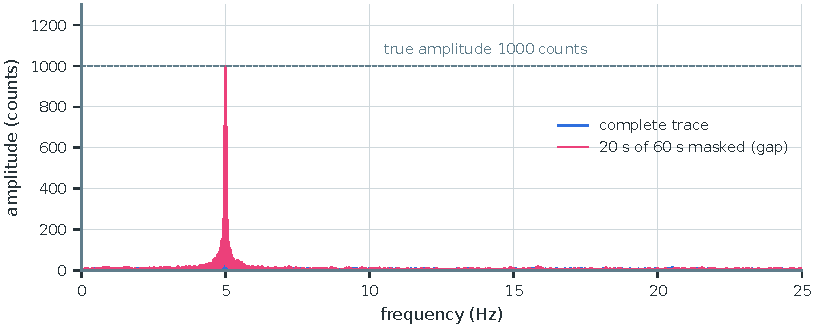
\includegraphics[width=\linewidth]{theory-amplitude-scaling}
\caption{Output of the application's \code{amplitude\_spectrum} for a 5~Hz sine of amplitude 1000~counts in noise,
with the trace complete (blue) and with 20~s of 60~s masked (pink). Both peak at 1000~counts.}\label{fig:ampscale}
\end{figure}

\section{Amplitude spectrum versus power spectral density}
An amplitude spectrum suits \emph{deterministic} signals such as tones, whose amplitude is meaningful. For
\emph{random} signals such as ground noise the meaningful quantity is the one-sided power spectral density (PSD),
the power per unit frequency. For a window $w$ the periodogram estimate is
\begin{equation}\label{eq:psd}
  S_{xx}[k] = \frac{2\,\abs{X_w[k]}^{2}}{\fs\sum_n w[n]^{2}}
  \qquad(\text{counts}^{2}/\text{Hz}),
\end{equation}
which integrates over frequency to the variance of the signal. The two are related, for a tone, by
$S_{xx}\,B_{\mathrm{ENBW}} = A^{2}/2$, where $B_{\mathrm{ENBW}}=\mathrm{ENBW}\cdot\df$ is the equivalent noise bandwidth in hertz. The Spectra mode shows amplitude; the spectrogram and the noise
spectrum (Chapters~\ref{ch:spectrogram} and~\ref{ch:noise}) show PSD in decibels.

\section{Variance of a spectrum estimate and why averaging helps}
The DFT of a random signal is itself random. For Gaussian noise the periodogram~\eqref{eq:psd} at a given frequency
is proportional to a $\chi^{2}$ variable with two degrees of freedom, whose standard deviation equals its mean:
the estimate does not become more reliable by making $N$ larger, it only becomes finer. This is the jagged look of a
single-window spectrum in \cref{fig:noisespec}.

\textcite{welch1967} reduced the variance by dividing the record into $K$ (possibly overlapping) segments,
computing a windowed periodogram of each, and averaging: the variance falls roughly as $1/K$ at the price of
resolution $K$ times coarser than the whole record would allow. The smooth blue curve in \cref{fig:noisespec} is the
root-mean-square average of 24 two-minute windows of the same night-time noise.

\begin{figure}[tbp]
\centering
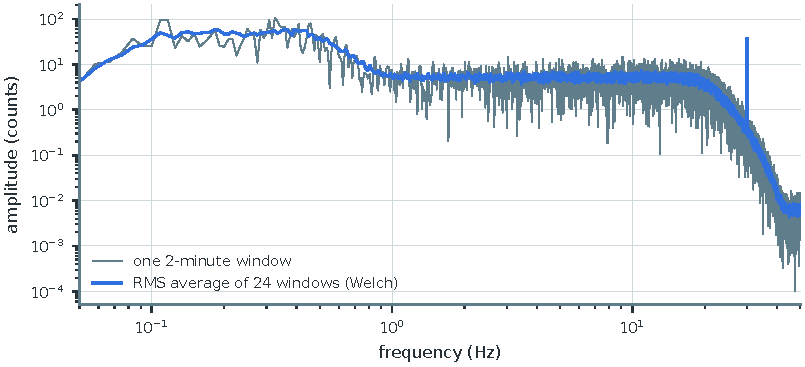
\includegraphics[width=\linewidth]{theory-noise-spectrum}
\caption{Amplitude spectrum of the night-time demo noise (EHZ, from 02:00~UTC). A single two-minute window (grey) is
jagged; the RMS average of 24 consecutive windows (blue) is smooth. The narrow line at 30~Hz is a deliberate
instrument line in the demo data.}\label{fig:noisespec}
\end{figure}

\begin{rs3dkey}
An amplitude spectrum is exact for tones and scaled by $2/\sum w$; a single-window spectrum of noise is always
jagged, and only averaging, as the spectrogram and noise spectrum do, makes it reliable.
\end{rs3dkey}

\chapter{The spectrogram}\label{ch:spectrogram}

A spectrum describes a whole window. Earthquakes, passing vehicles and instrument faults are \emph{events in time},
and an observer wants to see \emph{when} each frequency was present. The spectrogram answers this by computing a
spectrum for many short, overlapping windows and arranging them side by side.

\section{The short-time Fourier transform}
Choose a window of $N$ samples and a \emph{hop} of $H$ samples. The short-time Fourier transform (STFT) is
\begin{equation}\label{eq:stft}
  X[m,k] = \sum_{n=0}^{N-1} x[n+mH]\;w[n]\;e^{-\jj 2\pi k n/N},
\end{equation}
the DFT of the $m$-th windowed segment. Each segment is assigned the time of its \emph{centre}, $(mH+N/2)/\fs$ after the
start of the record. The spectrogram is the squared magnitude, converted to a power spectral density by~\eqref{eq:psd}
and to decibels:
\begin{equation}\label{eq:specdb}
  P[m,k] = 10\log_{10} S_{xx}[m,k]\qquad(\text{dB re. 1 count}^{2}/\text{Hz}).
\end{equation}
The overlap of consecutive windows is $N-H$; the application uses 50\,\%, so $H=N/2$.

\section{The time--frequency trade-off}
A window of length $T_w=N/\fs$ seconds has frequency resolution $\df = 1/T_w$ (Eq.~\ref{eq:resolution}) and time
resolution of about $T_w$. Making one finer makes the other coarser: it is not a limitation of the algorithm but of
physics, an instance of Gabor's uncertainty relation $\sigma_t\,\sigma_f \ge 1/4\pi$ \parencite{gabor1946}. \Cref{fig:tradeoff}
shows the same 90~s of the local earthquake with three window lengths. A 0.5~s window locates the P and S arrivals
sharply in time but cannot resolve frequency finer than 2~Hz; a 10~s window resolves 0.1~Hz but blurs the arrivals
over ten seconds.

\begin{figure}[tbp]
\centering
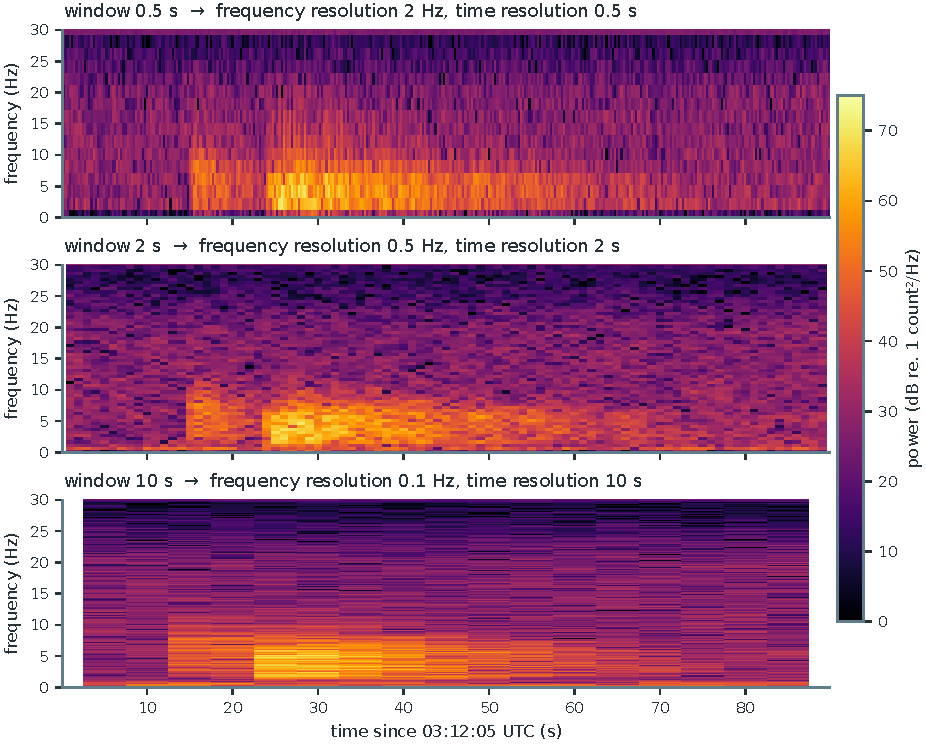
\includegraphics[width=\linewidth]{theory-spectrogram-tradeoff}
\caption{The demo local earthquake (EHZ, 03:12:05--03:13:35 UTC) with three window lengths, computed by the
application's \code{spectrogram}. Short windows localise the P and S onsets in time; long windows resolve
frequency.}\label{fig:tradeoff}
\end{figure}

\section{The window used by RS3D}
The application calls SciPy's \code{spectrogram} without specifying a window, so SciPy's default applies: a periodic
\textbf{Tukey window with $\alpha=0.25$}, which is flat in the middle and tapers with half-cosine edges over 25\,\% of the
window. \Cref{tab:windows} gives its measured properties: it is close to rectangular, with coherent gain $0.875$,
noise bandwidth $1.10$ bins, and a peak sidelobe only $-13.6$~dB below the peak. This is a defensible choice for
\emph{locating} events (the main lobe is narrow and little signal is lost) but it leaks more than the Hann window of the
amplitude spectrum.

\begin{rs3dwarn}[Leakage from strong low-frequency noise]
Because the Tukey window has high sidelobes that decay slowly, a very strong low-frequency signal, such as the
microseism, leaks a little energy into higher bins. For a typical RS3D day the effect is smaller than the dynamic range of the
colour scale, but a spectrogram of data with a large low-frequency component should be read with this in mind. Replacing the
window by a Hann window is a one-line change should it ever be needed.
\end{rs3dwarn}

\section{Choosing the window length: the 360 rule}
No single window length suits both a two-minute detail view and a 24-hour overview. The application chooses it from
the duration $T$ of the selection:
\begin{equation}\label{eq:window}
  T_w = \min\!\bigl(\max(T/360,\;1\ \mathrm{s}),\; 600\ \mathrm{s}\bigr).
\end{equation}
With 50\,\% overlap a record of duration $T$ yields about $2T/T_w-1\approx 719$ columns, a few hundred to a thousand, which
is about what a screen can display and what the browser can plot quickly, whatever the duration. The limits keep the
window between 1~s (so that even a short selection has a usable number of samples) and 10~minutes. \Cref{fig:rule} shows the
resulting window length and frequency resolution; \cref{tab:examples} gives worked examples.

\begin{figure}[tbp]
\centering
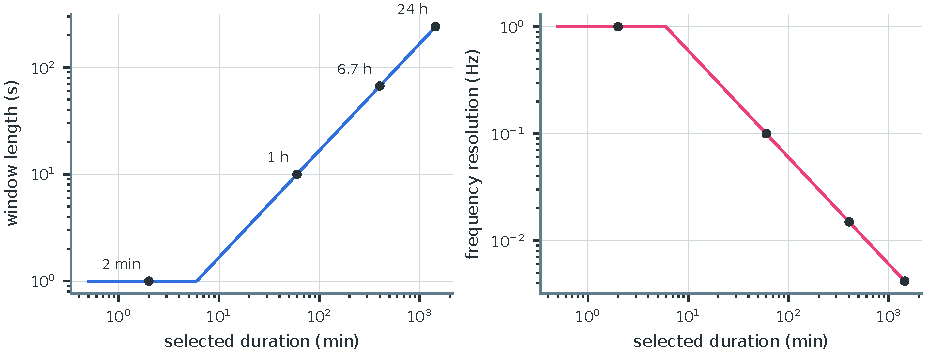
\includegraphics[width=\linewidth]{theory-window-rule}
\caption{The window-length rule~\eqref{eq:window} (left) and the frequency resolution it implies (right) as a function
of the selected duration.}\label{fig:rule}
\end{figure}

\begin{table}[tbp]
\centering\small
\caption{Window length, frequency resolution and number of columns for typical selections.}\label{tab:examples}
\begin{tabular}{@{}lrrr@{}}
\toprule
Selection & $T_w$ (s) & $\df$ (Hz) & columns\\ \midrule
2 minutes (detail view) & 1 & 1.0 & 239\\
1 hour & 10 & 0.1 & 719\\
6.7 hours & 67 & 0.015 & 719\\
24 hours & 240 & 0.004 & 719\\
\bottomrule
\end{tabular}
\end{table}

\section{Gaps}
A window that touches a gap would mix real signal with filler. The application therefore sets the samples of a gap to zero
for the transform and then marks \emph{every column whose window overlaps a gap} as not-a-number, drawn as blank. The
columns on either side of a gap are computed from complete windows only, so a gap does not smear into its
neighbours (\cref{fig:specday}, where two gaps are visible as white bars).

\section{From numbers to pixels}
The application never sends the full grid to the browser. The $(\text{frequency}\times\text{time})$ matrix is
\emph{binned} to at most $400\times200$ cells; each cell shows the mean of the decibel values it covers, and cells with no
valid value are left out. Averaging \emph{decibels} is the same as taking a geometric mean of power, which slightly
underestimates narrow peaks compared with averaging power. The colour scale runs from the 2nd to the 98th percentile of
the displayed values, so that a few extreme cells do not wash out the picture.

\begin{figure}[tbp]
\centering
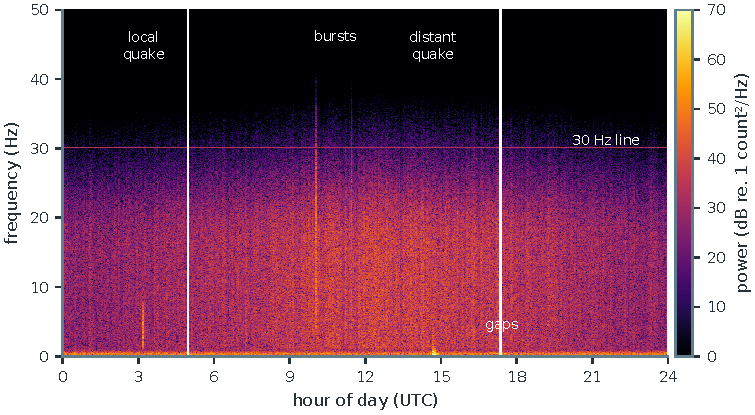
\includegraphics[width=\linewidth]{theory-spectrogram-day}
\caption{A full-day spectrogram of the demo EHZ channel computed with the application's functions (window 240~s). The
day--night change in cultural noise, the local and distant earthquakes, two noise bursts, the 30~Hz instrument line and the
two gaps (white) are all visible.}\label{fig:specday}
\end{figure}

\section{Reading a spectrogram}
\begin{description}[leftmargin=2.2cm,style=nextline]
\item[Earthquake] a vertical streak starting abruptly at the P arrival; energy at higher frequencies arrives first and the
  S wave follows, with a coda fading at lower frequencies.
\item[Man-made burst] a short, broadband streak with no coda; compare the two bursts at about 10--11~h in
  \cref{fig:specday}.
\item[Narrow horizontal line] a persistent single frequency: usually electrical interference or machinery, here the
  30~Hz instrument line.
\item[Slow day--night change] cultural noise, strongest in working hours.
\item[Low-frequency band] the ocean microseism, near 0.1--0.3~Hz.
\end{description}

\begin{rs3dapp}
\code{spectrogram(trace, window\_s, overlap=0.5)} in \file{core/spectro.py} returns window-centre times, frequencies and
decibel values; \code{window\_for(duration)} is Eq.~\eqref{eq:window}. The page code
(\file{app/charts.py}, \code{spectrogram\_options}) performs the binning and colour scaling.
\end{rs3dapp}

\chapter{The noise spectrum}\label{ch:noise}

The \ui{Noise spectrum} panel on the Data page summarises how much energy the ground contained at each frequency during
the selected time, as a median curve with a band around it. It is the quickest way to judge a site, to compare day with
night, and to spot a new source of interference.

\section{Definition}
Start from the spectrogram grid $P[m,k]$ of Eq.~\eqref{eq:specdb} (columns $m$ are times, rows $k$ frequencies).
\begin{enumerate}
\item Drop every column that is entirely not-a-number, that is, every window touching a gap.
\item Drop the zero-frequency row.
\item For each frequency $f_k$ compute three \emph{percentiles} across the remaining columns:
  \[
    P_{10}[k],\qquad P_{50}[k]=\median_m P[m,k],\qquad P_{90}[k].
  \]
\end{enumerate}
The panel draws $P_{50}$ as a line and the range $P_{10}$--$P_{90}$ as a band on a logarithmic frequency axis.

Percentiles, and not the mean, are used because they are \emph{robust}: an earthquake or a noise burst occupies a small
fraction of the columns, so it moves $P_{90}$ but leaves the median essentially at the level of the background
noise. \Cref{fig:psd} compares one night hour with one midday hour of the demo day.

\begin{figure}[tbp]
\centering
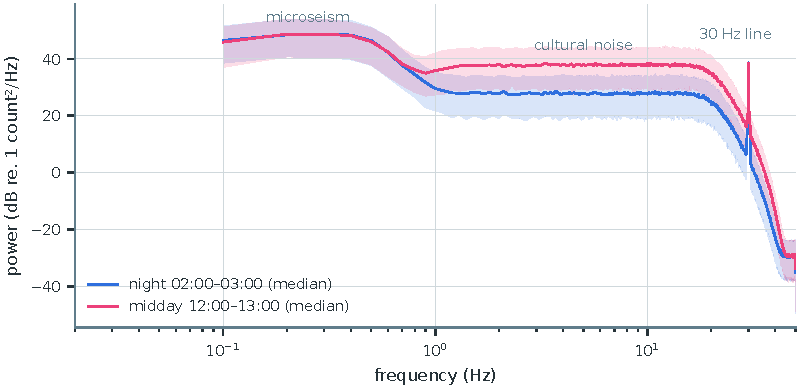
\includegraphics[width=\linewidth]{theory-psd-summary}
\caption{Noise spectrum of the demo EHZ channel for 02:00--03:00 (blue) and 12:00--13:00 (pink): median and
10th--90th percentile band, from the application's \code{spectrogram} and \code{psd\_summary}. Cultural noise above
1~Hz is clearly stronger at midday.}\label{fig:psd}
\end{figure}

\section{Relation to the McNamara--Buland PPSD}
The standard tool for describing the noise of a seismic station is the \emph{probabilistic power spectral density}
(PPSD) of \textcite{mcnamara2004}. Its recipe is: cut the data into one-hour segments; estimate a PSD for each with
Welch's method, correct it for the instrument response; smooth it into narrow period bands; and accumulate, for every
period, a histogram of the resulting power levels. The histograms, together with the global new low-noise and
high-noise models of \textcite{peterson1993}, show at a glance how quiet and how variable a site is.

The noise spectrum of RS3D is a deliberately simplified relative of the PPSD, and the differences matter when the
two are compared.

\begin{table}[tbp]
\centering\small
\caption{RS3D noise spectrum versus the PPSD of McNamara and Buland (2004).}\label{tab:ppsd}
\begin{tabular}{@{}L{0.23\linewidth}L{0.35\linewidth}L{0.35\linewidth}@{}}
\toprule
 & PPSD & RS3D noise spectrum\\ \midrule
Segments & one-hour, overlapping & the spectrogram windows of the chosen range\\
Averaging inside a segment & Welch average of sub-segments & none: each window is one periodogram\\
Instrument response & removed & \textbf{not} removed (counts$^2$/Hz)\\
Frequency smoothing & narrow octave fractions & none (linear bins)\\
Summary & full histogram per period & 10th, 50th and 90th percentile\\
Reference models & NLNM and NHNM & none\\
\bottomrule
\end{tabular}
\end{table}

\begin{rs3dwarn}[Not comparable with the Peterson noise models]
Because the response is not removed, the RS3D curve is in counts$^2$/Hz, not in the acceleration units of the
Peterson models, and its shape includes the geophone's own roll-off below 4.5~Hz. It must be used for
\emph{relative} comparisons on the same instrument (day versus night, this week versus last week), not to rank a site
against published noise levels.
\end{rs3dwarn}

\section{What the curves tell you}
\begin{description}[leftmargin=2.2cm,style=nextline]
\item[Microseism, 0.1--0.3~Hz] ocean waves coupling to the sea floor; present everywhere, strongest in winter storms. A
  short-period geophone sees it faintly because its response falls steeply below 4.5~Hz.
\item[Above 1~Hz] cultural noise (traffic, machinery, people). It changes with the time of day and the day of the week;
  the difference between the two curves of \cref{fig:psd} is a direct measure of it.
\item[Narrow peaks] a single frequency that never changes: interference. The 30~Hz line of the demo data is an example.
\item[Roll-off near 50~Hz] the digitiser's anti-alias filter (Chapter~\ref{ch:data}); it is a property of the instrument,
  not of the ground.
\end{description}

\begin{rs3dapp}
\code{psd\_summary(freqs, power\_db)} in \file{core/spectro.py} returns $(f, P_{10}, P_{50}, P_{90})$ using
\code{numpy.percentile} on the decibel values, after dropping gap columns and the zero-frequency bin. The chart is
\code{psd\_options} in \file{app/charts.py}.
\end{rs3dapp}

\chapter{Data quality: gaps and completeness}\label{ch:quality}

A seismograph is only useful while it is recording. The application measures and displays three aspects of
\emph{data availability}: what is on the laptop and what is still on the Shake (the coverage bar), what is missing
inside the selected window (Data health), and whether the Shake's clock can be trusted (Chapter~\ref{ch:data}).

\section{Samples, spans and gaps}
A trace is a set of samples at times $t_i=t_0+i/\fs$. Records and traces end where a gap begins, so the whole day is a
list of \emph{spans} $[s_j,e_j)$, where $e_j$ is the time just after the last sample of the span, $e_j=s_j+N_j/\fs$. Two
spans are \emph{contiguous} when the hole between them is at most half a sample, which absorbs timing rounding;
contiguous spans are merged. What counts as a gap depends on who is asking, so the application uses three tolerances.

\begin{table}[tbp]
\centering\small
\caption{Gap tolerances used by different parts of the application.}\label{tab:tol}
\begin{tabular}{@{}L{0.34\linewidth}cL{0.46\linewidth}@{}}
\toprule
Use & Tolerance & Rule\\ \midrule
Coverage bar (\file{core/coverage.py}) & $0.5/\fs$ & spans closer than half a sample are merged into one\\
Data health (\file{core/health.py}) & $0.5/\fs$ & same rule, applied per channel\\
Helicorder rows (\file{core/helicorder.py}) & $1.5/\fs$ & a break is drawn only when the hole exceeds one and a
  half sample intervals\\
\bottomrule
\end{tabular}
\end{table}

\section{Completeness}
For a selection $[a,b)$ with $\Tsel=b-a$ the application computes, for every channel, the set of times with data (the union
of its clipped spans) and from it the set of times \emph{missing} on that channel. The \emph{gaps} of the selection are the
union, over channels, of the missing sets: a moment counts as a gap if \emph{any} selected channel has no data. The
\emph{completeness} is
\begin{equation}\label{eq:complete}
  C = 1-\frac{\sum_g (e_g - s_g)}{\Tsel}, \qquad 0\le C\le1,
\end{equation}
where the sum runs over the gaps $g$ of the union. If no channel has any data in the selection there is one gap equal to
the whole selection and $C=0$. \Cref{fig:gaps} illustrates the construction.

\begin{figure}[tbp]
\centering
\begin{tikzpicture}[x=0.078\linewidth,y=1cm]
  \foreach \y/\lab/\spans in {2.4/EHZ/{0/3.2, 4.0/10},1.6/EHN/{0/10},0.8/EHE/{0/6.1, 6.7/10}} {
    \node[left,font=\small\sffamily] at (-0.15,\y) {\lab};
    \foreach \a/\b in \spans { \fill[rs3dblue!70] (\a,\y-0.22) rectangle (\b,\y+0.22); }
  }
  \node[left,font=\small\sffamily] at (-0.15,0) {union};
  \fill[rs3dred!70] (3.2,-0.22) rectangle (4.0,0.22);
  \fill[rs3dred!70] (6.1,-0.22) rectangle (6.7,0.22);
  \draw[rs3dgrey] (0,-0.6) -- (10,-0.6);
  \foreach \x/\t in {0/$a$,10/$b$} {\draw[rs3dgrey] (\x,-0.5) -- (\x,-0.7); \node[below,font=\small] at (\x,-0.7) {\t};}
  \node[font=\small,rs3dred!80!black,above] at (3.6,0.25) {$g_1$};
  \node[font=\small,rs3dred!80!black,above] at (6.4,0.25) {$g_2$};
  \draw[decorate,decoration={brace,amplitude=3pt,mirror},rs3dgrey] (0,-1.15) -- (10,-1.15)
    node[midway,below=3pt,font=\small] {$\Tsel$};
\end{tikzpicture}
\caption{Completeness of a selection. Each channel has its own holes; the gaps of the selection ($g_1$, $g_2$) are the
union of all of them, and $C=1-(|g_1|+|g_2|)/\Tsel$. In this sketch $C = 1-(0.8+0.6)/10 = 86\,\%$.}\label{fig:gaps}
\end{figure}

\begin{rs3dapp}
\code{health(stream, start, end)} in \file{core/health.py} returns the completeness and the list of gaps, each as a
pair of times; the Data page prints it as a percentage and lists up to 50 gaps with their durations in the chosen
time zone. The leading and trailing holes of a selection (data starting after $a$ or ending before $b$) are gaps like
any other.
\end{rs3dapp}

\section{Coverage: laptop, Shake, or nothing}
The coverage bar above the Data page's preview classifies every instant of a view into three states:
\emph{local} (the samples are on the laptop), \emph{remote} (the day exists on the Shake but is not downloaded) and
\emph{gap} (no data anywhere). The rule, evaluated per segment between cut points at midnight and at span edges, is:
\begin{enumerate}
\item if the midpoint of the segment lies inside a local span, the state is local;
\item otherwise, if that day exists on the Shake \emph{and} the laptop does not have the day file, or the day is the newest day
  on the Shake (still being written), the state is remote;
\item otherwise it is a gap.
\end{enumerate}
The ``newest day'' exception is why today's file is always offered for download again: the Shake appends to it
continuously, so a copy made earlier is incomplete.

\section{Why a gap is never filled}
Interpolating across a gap would be easy and would make plots prettier, but it would manufacture data. RS3D keeps gaps as
gaps in every stage: separate traces on loading, separate filter runs, \code{NaN} separators in the plotted lines, blank
spectrogram columns, and an explicit completeness figure. When a gap is shorter than the window of an operation, that
operation excludes the window rather than guessing its content.

\chapter{Visualisation algorithms}\label{ch:vis}

One day of one channel is $86400\times100=8.64$ million samples; a screen is a few thousand pixels wide. Every plot of
RS3D therefore \emph{reduces} the data before drawing it. How it is reduced decides whether a short, important spike
survives. This chapter describes the reductions and the geometry of the helicorder.

\section{Reducing a signal for display}
\subsection{Stride decimation and why it can lose a spike}
The simplest reduction keeps every $q$-th sample. It is fast, and for a signal that is oversampled relative to its
bandwidth it is harmless, but for a spiky signal it is wrong: the sampling theorem (Chapter~\ref{ch:data}) applies again,
and a feature narrower than $q$ samples is either kept or discarded depending on where it falls in the grid.
\Cref{fig:minmax} (middle) shows a one-sample spike that stride decimation misses.

\subsection{Min/max decimation}
A seismogram plot is read mainly through its \emph{envelope}, the extremes within each short interval. Min/max
decimation preserves exactly that. The record is divided into $B$ consecutive bins; from each bin the algorithm keeps
the sample with the smallest value and the sample with the largest value (one point if they coincide), in time order.
The plot then has at most $2B$ points and contains the true extremes of every bin:
\begin{equation}\label{eq:minmax}
  \bigl(t^{\min}_b,\,x^{\min}_b\bigr),\ \bigl(t^{\max}_b,\,x^{\max}_b\bigr),\qquad
  x^{\min}_b=\min_{n\in b}x[n],\quad x^{\max}_b=\max_{n\in b}x[n].
\end{equation}
Peak amplitudes and their times are therefore \emph{exact}; what is lost is the detailed shape inside a bin, which
is below the pixel resolution anyway. The cost is linear in the number of samples.

\begin{figure}[tbp]
\centering
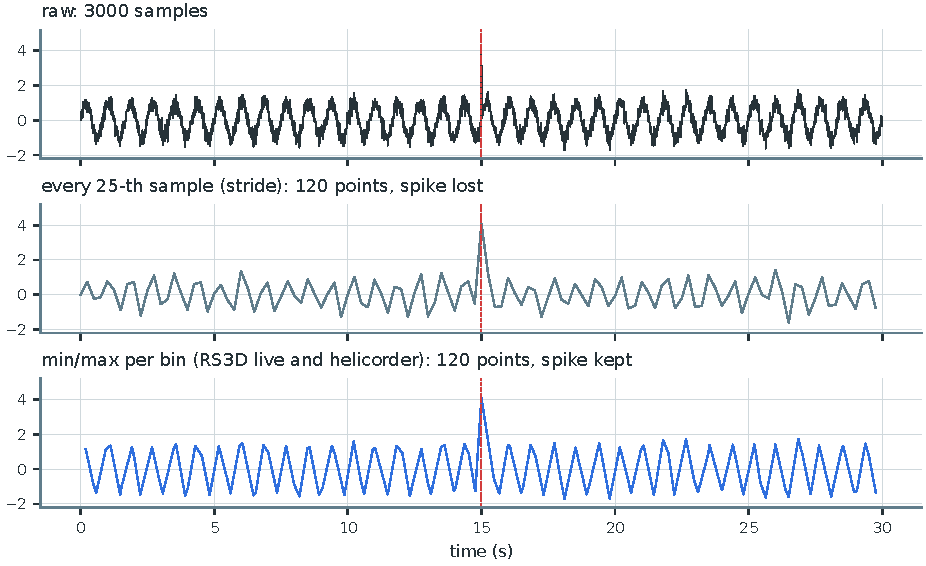
\includegraphics[width=\linewidth]{theory-minmax}
\caption{Reducing 3000 samples to 120 points. Top: the raw signal with one single-sample spike (dashed line).
Middle: every 25th sample, which misses the spike. Bottom: min/max decimation as implemented in
\code{minmax\_decimate}, which keeps it.}\label{fig:minmax}
\end{figure}

\paragraph{Gaps.} The input to the decimator marks gaps with \code{NaN} samples. The record is first split at these
markers, each segment is decimated on its own with a share of the point budget proportional to its length (at least one
bin), and a \code{NaN} is re-inserted between segments, so the plotted line breaks at every gap and no line is drawn
across missing data.

\begin{rs3dapp}
\code{minmax\_decimate(t, v, max\_points)} in \file{core/live.py} is used by the Live view (up to 1500 points per
channel) and by the helicorder (3000 points per row, \code{POINTS\_PER\_ROW}). \textbf{The waveform preview on the Data page
and the detail view are different:} \code{set\_stream\_data} in \file{app/charts.py} thins each trace with a stride of
$\lceil N/4000\rceil$ and then lets the charting library apply its own ``largest-triangle-three-buckets'' downsampling
\parencite{steinarsson2013}, which also preserves visual shape but does not guarantee exact extremes. For the short
windows of the detail view (a few thousand samples) no reduction occurs at all, so the issue arises only for long
previews. Moving the preview to min/max decimation would be a straightforward improvement.
\end{rs3dapp}

\section{The helicorder}
A helicorder (from \emph{helical recorder}) wraps a long record into rows, like lines of text, so that a day fits on one
page and an event stands out as a burst on one line.

\subsection{Geometry}
Let $t_0$ be midnight UTC, $\Delta=1800$~s the row length (30 minutes) and $R=48$ the number of rows. Row $i$ shows the
interval $[t_0+i\Delta,\ t_0+(i+1)\Delta)$. A sample at time $t$ in row $i$ is drawn at horizontal position
\begin{equation}
  x = \frac{t-(t_0+i\Delta)}{60}\quad\text{minutes},\qquad 0\le x<30,
\end{equation}
and vertical position
\begin{equation}\label{eq:heliy}
  y = i - \frac{v(t)-m_i}{S},
\end{equation}
with the $y$ axis pointing down, so a positive excursion moves the trace up. Here $m_i$ is the \emph{median} of row $i$ and
$S$ is a single amplitude scale shared by all rows.

\subsection{Removing the offset}
Raw counts sit on a DC offset (Chapter~\ref{ch:response}). Without $m_i$ the offset divided by $S$ would shift each row
by a fixed fraction of a row, and, worse, would enter the scale $S$ (below), flattening the signal.
\Cref{fig:dcoffset} contrasts the two. The median is used because, unlike the mean, it is not pulled by an earthquake
inside the row.

\begin{figure}[tbp]
\centering
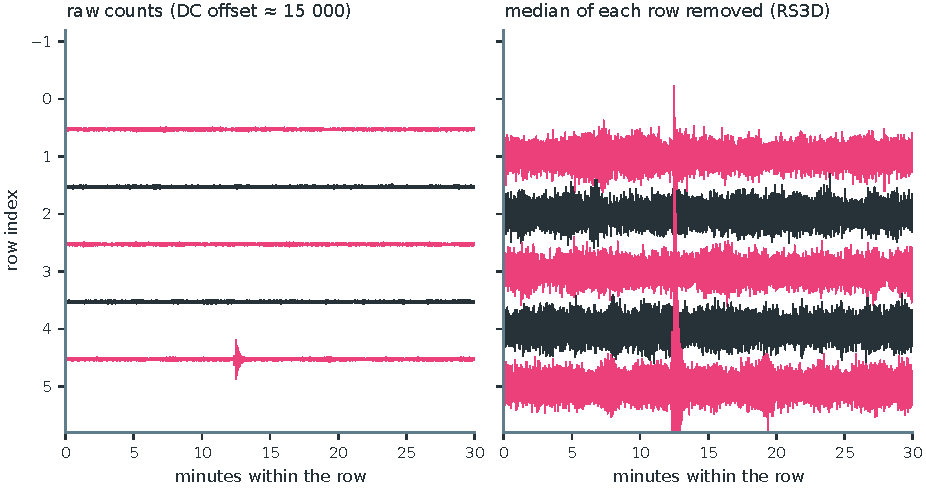
\includegraphics[width=\linewidth]{theory-dc-offset}
\caption{Six rows of the demo EHZ channel with an offset of about 15\,000~counts. Left: raw counts: the offset
dominates the scale and every trace is a nearly flat line shifted by half a row. Right: the median of each row removed:
the signal fills the row height and the small local earthquake is visible in the lower rows.}\label{fig:dcoffset}
\end{figure}

\subsection{The amplitude scale}
The scale $S$ decides how tall the traces are. It must be large enough that adjacent rows do not collide and small
enough that quiet signals are visible. The application sets
\begin{equation}\label{eq:scale}
  S = \frac{2\,P_{99}\bigl(\,\abs{v_{\mathrm{dec}}-m}\,\bigr)}{F},
\end{equation}
where $P_{99}$ is the 99th percentile of the absolute values of all plotted (decimated, median-removed) points of the
day, and $F$ is the user's \ui{Scale} factor ($0.5\times$ to $8\times$). With $F=1$, the 99th percentile maps to half a
row, so ordinary signal fills about one row and only the strongest 1\,\% exceed it. A percentile is used rather than the
maximum so that one huge event does not squash a whole quiet day into flat lines. Note that because the points are min/max
extrema, $P_{99}$ of the decimated data is somewhat larger than that of the raw samples.

\begin{figure}[tbp]
\centering
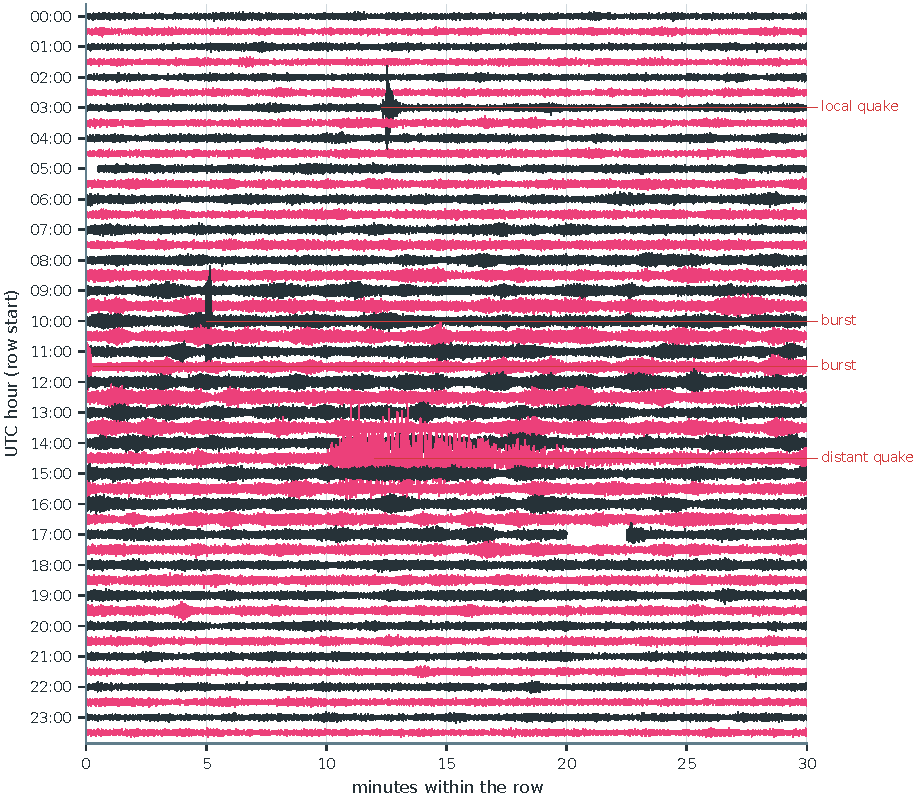
\includegraphics[width=0.92\linewidth]{theory-helicorder}
\caption{A day of the demo EHZ channel drawn with the application's \code{build\_rows} and \code{scale\_for}. Rows are
30~minutes; the day--night change, the local earthquake (03:00 row), two noise bursts, the distant earthquake
(14:30 row) and a gap at 17:20 are visible.}\label{fig:heli}
\end{figure}

\subsection{From a click to a time}
The helicorder page must convert a mouse click into a time. ECharts reports clicks on \emph{data points}, not on empty
space, so the page lays an invisible grid of $48\times180$ points over the plot: one every 10~seconds along each row, drawn as
transparent $10\times14$ pixel rectangles. A click reports the nearest grid point as the pair
$(x_{\min},\,i)$, and the time is
\begin{equation}\label{eq:click}
  t = t_0 + \Delta\left(i + \frac{x_{\min}}{30}\right),\qquad x_{\min}\ \text{clamped to}\ [0,30].
\end{equation}
Equation~\eqref{eq:click} (\code{click\_to\_time} in \file{core/helicorder.py}) is exact for the grid point; the point
itself is at most 5~s from where the pointer was. The chart height is fixed to $48\times14+44$~pixels so that each row is
exactly 14 pixels and a pixel row corresponds to a row index without rounding.

\section{The detail view}
A click opens a window of $T_w=120$~s centred on the clicked time. The toolbar changes this window with a small set of
pure functions (\file{core/helicorder.py}):
\begin{description}[leftmargin=2.4cm,style=nextline]
\item[Zoom out / in] multiplies the span by 2 or $\tfrac12$ about the centre, clamped to between 5 and 3600 seconds.
\item[Earlier / later] shifts the window by $\mp\tfrac12$ of its span.
\item[Box zoom] a dragged rectangle gives a time interval $[x_0,x_1]$ (epoch ms) and an amplitude interval. The new window is
  the rectangle's time span clipped to the current window and widened, centred, to at least 5~s; a rectangle that does not
  overlap the window changes nothing. The amplitude interval, rounded to four significant figures for readable axis
  labels, fixes the vertical axis.
\item[Fit] clears any amplitude zoom, so the axis rescales to the data in view; the time window is kept.
\end{description}

\begin{rs3dkey}
Min/max decimation keeps peaks exact; the helicorder removes each row's median and scales all rows by the same robust
percentile; a click becomes a time through a 10-second grid.
\end{rs3dkey}

\chapter{Event detection and alerts}\label{ch:detect}

An observer cannot watch a screen all day. The purpose of an \emph{alert} is to say, without a human present, that
something happened: the ground moved more than it normally does. This chapter explains the standard way of
deciding that, the STA/LTA trigger \parencite{allen1978}, shows how it behaves on data whose true events are known,
and describes how RS3D's alert pipeline is designed around it.

\begin{rs3dwarn}[Status of this chapter]
Sections~\ref{sec:detprob} to~\ref{sec:failures} describe standard theory and measurements made with the
application's demo data and ObsPy's reference implementation. Section~\ref{sec:alertdesign} is a \emph{design proposal}: the alert feature
of RS3D is not yet implemented, and the proposal will be revised after it is.
\end{rs3dwarn}

\section{The detection problem}\label{sec:detprob}
Detection is a decision between two hypotheses at every instant: $H_0$, \emph{only background noise}, and $H_1$, \emph{noise
plus a seismic signal}. Any decision rule makes two kinds of mistakes: a \emph{false alarm} (declaring $H_1$ when $H_0$ is
true) and a \emph{missed detection} (declaring $H_0$ when $H_1$ is true). Lowering the threshold at which an event is
declared catches weaker events but raises the false-alarm rate, and vice versa; no rule escapes the trade-off, and the art
lies in choosing a rule whose false alarms are rare enough to tolerate at an acceptable sensitivity. For an alert that wakes
somebody at night the tolerable false-alarm rate is very low.

The difficulty is that seismic noise is not a fixed distribution. It changes with the time of day, the weather and the
neighbours' habits. A detector must therefore compare the \emph{present} signal with the \emph{recent} noise level,
not with a constant. This is the idea of the STA/LTA trigger.

\section{The characteristic function}\label{sec:cf}
Before averaging, the signal is turned into a non-negative \emph{characteristic function} (CF) $c[n]$ that grows when a signal is
present. The simplest choices are the squared amplitude, $c[n]=x[n]^{2}$ (an instantaneous power), or the absolute value
$\abs{x[n]}$. Allen's original function also includes the squared first difference, which responds to
abrupt changes. ObsPy's reference implementation, and RS3D's design, use $c[n]=x[n]^{2}$.

Two preprocessing steps are essential before the CF is formed.
\begin{enumerate}
\item \textbf{Remove the offset.} The DC component of raw counts (Chapter~\ref{ch:response}) would be squared into a huge
  constant that masks any event. A band-pass filter that rejects frequencies below the lower corner removes it.
\item \textbf{Band-pass filter, causally.} Restricting the signal to the band where the events of interest have their
  energy raises the signal-to-noise ratio. For the filter to be usable in real time and not to blur the onset
  (Chapter~\ref{ch:filter}) it must be \emph{causal}.
\end{enumerate}

\section{The classic STA/LTA}
Let $N_s$ and $N_l$ be the lengths, in samples, of a short and a long window, $N_s\ll N_l$. The short-term average (STA) and
long-term average (LTA) of the CF at sample $i$ are the means over the two \emph{trailing} windows:
\begin{equation}\label{eq:stalta}
  \mathrm{STA}_i = \frac{1}{N_s}\sum_{j=i-N_s+1}^{i} c[j],\qquad
  \mathrm{LTA}_i = \frac{1}{N_l}\sum_{j=i-N_l+1}^{i} c[j],\qquad
  R_i = \frac{\mathrm{STA}_i}{\mathrm{LTA}_i}.
\end{equation}
The STA follows the signal quickly and estimates the \emph{current} power; the LTA changes slowly and estimates the
\emph{background}. In quiet noise $R\approx1$. When an event arrives the STA rises almost at once while the LTA, which
averages over a long past, hardly moves, so $R$ jumps. The detector declares an event when $R$ crosses a
\emph{trigger-on threshold} $r_{\mathrm{on}}$ upward and ends it when $R$ falls below a lower \emph{trigger-off threshold}
$r_{\mathrm{off}}<r_{\mathrm{on}}$. Using two thresholds, \emph{hysteresis}, prevents rapid on--off flicker when $R$
hovers near one value.

\begin{figure}[tbp]
\centering
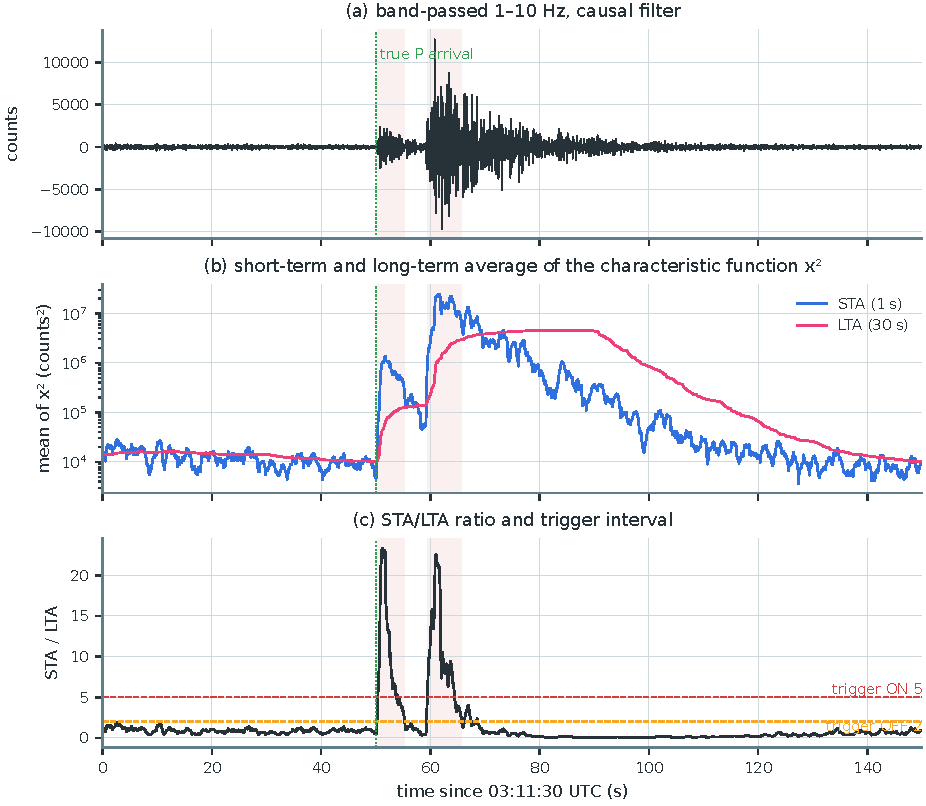
\includegraphics[width=\linewidth]{theory-stalta-example}
\caption{STA/LTA on the demo local earthquake (EHZ). (a) The signal band-passed 1--10~Hz with a causal filter. (b) STA (1~s)
and LTA (30~s) of the characteristic function $x^{2}$: the STA jumps by orders of magnitude at the P arrival while the LTA
lags. (c) The ratio, the thresholds ($r_{\mathrm{on}}=5$, $r_{\mathrm{off}}=2$) and the trigger intervals (pink). The ratio
falls back below the threshold between the P and the S wave, so the single earthquake produces two trigger intervals.}\label{fig:stalta}
\end{figure}

\subsection{The warm-up period}
$\mathrm{LTA}_i$ is meaningless until $N_l$ samples have been seen. ObsPy sets the ratio to zero for the first samples; a
live monitor must not raise an alert during this period, which is $N_l/\fs$ seconds long (30~s in the example).

\section{The recursive STA/LTA}
The classic form needs the last $N_l$ samples in memory. A \emph{recursive} variant replaces each moving average by an
exponential one:
\begin{equation}\label{eq:rec}
  \mathrm{STA}_i = \mathrm{STA}_{i-1} + \frac{c[i]-\mathrm{STA}_{i-1}}{N_s},\qquad
  \mathrm{LTA}_i = \mathrm{LTA}_{i-1} + \frac{c[i]-\mathrm{LTA}_{i-1}}{N_l}.
\end{equation}
Unrolling the recursion shows that sample $c[i-k]$ carries the weight $\frac1N(1-\frac1N)^k$: a geometric, not a
rectangular, window, with a \emph{time constant} of $N$ samples ($\tau_s=N_s/\fs$, $\tau_l=N_l/\fs$ seconds)
\parencite{withers1998,trnkoczy2012}. The recursion needs only two numbers of state and one multiplication per sample,
independent of $N_l$, which makes it the natural choice for a monitor that runs continuously on a stream.
For the same $N_s$ and $N_l$ the two forms give similar but not identical ratios.

\section{Setting the parameters}\label{sec:params}
The three groups of parameters have different roles; \textcite{trnkoczy2012} gives a systematic treatment.

\begin{description}[leftmargin=2.2cm,style=nextline]
\item[STA length] should be a few periods of the dominant signal frequency: long enough that the STA is not driven by a
  single large sample, short enough to react quickly. A short STA finds short, impulsive events; a long STA favours
  emergent ones. \Cref{fig:params} (left) shows the effect.
\item[LTA length] should be much longer than the STA (a factor of 10 or more) so that an event does not contaminate its own
  background estimate, yet short enough to follow the slow change of the noise. \Cref{fig:params} (right) shows the
  effect.
\item[Thresholds] $r_{\mathrm{on}}$ sets the sensitivity; $r_{\mathrm{off}}$, typically a fraction of $r_{\mathrm{on}}$, sets how
  long an event is held. The values of the example, $r_{\mathrm{on}}=5$ and $r_{\mathrm{off}}=2$, were chosen from the sweep of
  \cref{fig:sweep}.
\item[Pass band] the band in which the CF is formed; it should contain the energy of the target events and exclude
  the dominant noise.
\end{description}

\begin{figure}[tbp]
\centering
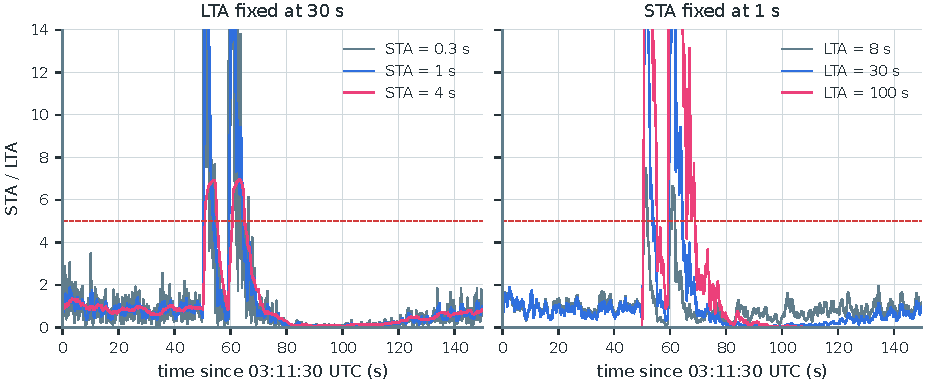
\includegraphics[width=\linewidth]{theory-stalta-params}
\caption{Effect of the window lengths on the ratio for the same earthquake. Left: STA of 0.3, 1 and 4~s with LTA 30~s. A
longer STA gives a lower, smoother peak. Right: LTA of 8, 30 and 100~s with STA 1~s. A short LTA is contaminated by the
event itself and the ratio collapses quickly. Dashed: threshold 5.}\label{fig:params}
\end{figure}

\subsection{Statistical meaning of the ratio}
If the signal is Gaussian noise and the CF is $x^{2}$, the average of $x^{2}$ over a window follows a scaled $\chi^{2}$
distribution. For noise that occupies a bandwidth $B$ (hertz) a window of $T$ seconds contains about $\nu\approx 2BT$
independent values, so STA and LTA have $\nu_s=2BT_s$ and $\nu_l=2BT_l$ degrees of freedom and, for stationary noise, the ratio $R$
follows an $F$ distribution with $(\nu_s,\nu_l)$ degrees of freedom. For the 1--10~Hz band ($B\approx9$~Hz) with a 1~s STA and a
30~s LTA this gives $\nu_s=18$ and $\nu_l=540$. The probability that a \emph{single} ratio value exceeds a threshold is then
tiny (\cref{tab:null}, second column): $1.4\times10^{-10}$ at $r=5$.

\begin{table}[tbp]
\centering\small
\caption{False alarms per day (events merged within 30~s) for stationary Gaussian noise and for the demo day, with the
$F$-distribution tail probability for one independent ratio value. Detector: causal 1--10~Hz band-pass, recursive STA/LTA,
STA 1~s, LTA 30~s, $r_{\mathrm{off}}=0.4\,r_{\mathrm{on}}$.}\label{tab:null}
\begin{tabular}{@{}rrrr@{}}
\toprule
Threshold & F tail $P(R>r)$ & Stationary noise & Demo day \\ \midrule
2 & 8.5e-03 & 89 & 498 \\
2.5 & 6.0e-04 & 0 & 240 \\
3 & 3.5e-05 & 0 & 83 \\
3.5 & 1.7e-06 & 0 & 25 \\
4 & 7.9e-08 & 0 & 7 \\
5 & 1.4e-10 & 0 & 0 \\
6 & 2.3e-13 & 0 & 0 \\
\bottomrule
\end{tabular}

\end{table}

The table's last two columns are the important result. For \emph{stationary} noise, false alarms disappear
above $r\approx 2.5$, as theory predicts. The demo day, whose noise changes with the time of day and fluctuates from
minute to minute, still produces 83 false events per day at $r=3$ and does not reach zero until $r=5$.
\emph{Real noise is not stationary}, the LTA lags behind every rise in the noise level, and a threshold chosen from
stationary theory is far too sensitive.

\begin{figure}[tbp]
\centering
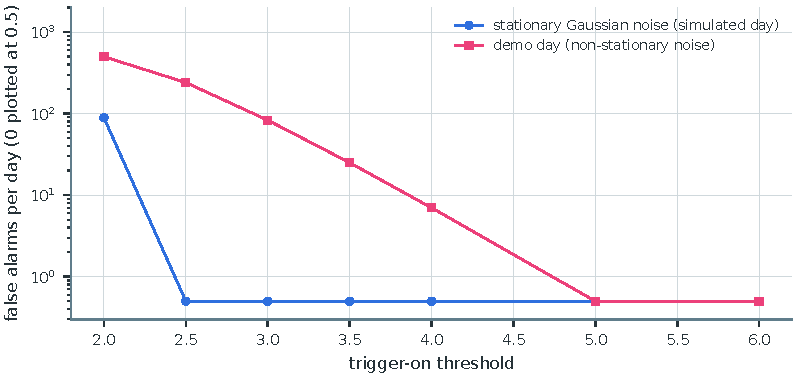
\includegraphics[width=\linewidth]{theory-stalta-null}
\caption{False alarms per day against threshold for stationary noise (blue) and the demo day (pink); zeros are plotted at
0.5 on the logarithmic axis.}\label{fig:null}
\end{figure}

\begin{rs3dkey}
The threshold must be chosen from the noise of \emph{your} site, over days, not from the theory of stationary noise.
A threshold that gives zero false alarms on stationary noise may give dozens per day on a real station.
\end{rs3dkey}

\section{Behaviour on the demo day}\label{sec:demoday}
\Cref{fig:staltaday} applies the detector (causal 1--10~Hz band-pass, recursive STA/LTA, STA 1~s, LTA 30~s,
$r_{\mathrm{on}}=5$, $r_{\mathrm{off}}=2$, events closer than 30~s merged) to the whole demo day. \Cref{tab:events}
lists the events found. All three are real in the sense that something happened; two of them are not earthquakes.

\begin{figure}[tbp]
\centering
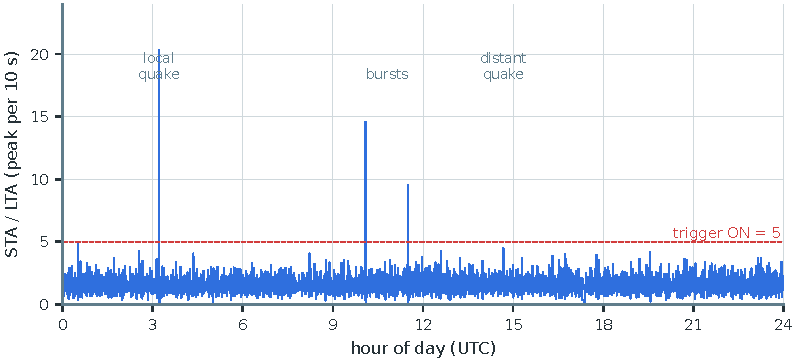
\includegraphics[width=\linewidth]{theory-stalta-day}
\caption{The STA/LTA ratio over the demo day (peak per 10~s). Three episodes cross the threshold of 5: the local earthquake
and the two noise bursts. The distant earthquake, whose energy is below 1~Hz, stays below it.}\label{fig:staltaday}
\end{figure}

\begin{table}[tbp]
\centering\small
\caption{Events detected on the demo day at $r_{\mathrm{on}}=5$. The ``cause'' is known because the demo data were constructed.}\label{tab:events}
\begin{tabular}{@{}lrrl@{}}
\toprule
Onset (UTC) & Duration (s) & Peak ratio & Cause \\ \midrule
03:12:20 & 18 & 20.3 & local earthquake \\
10:05:00 & 12 & 14.6 & noise burst \\
11:30:00 & 12 & 9.5 & noise burst \\
\bottomrule
\end{tabular}

\end{table}

\begin{figure}[tbp]
\centering
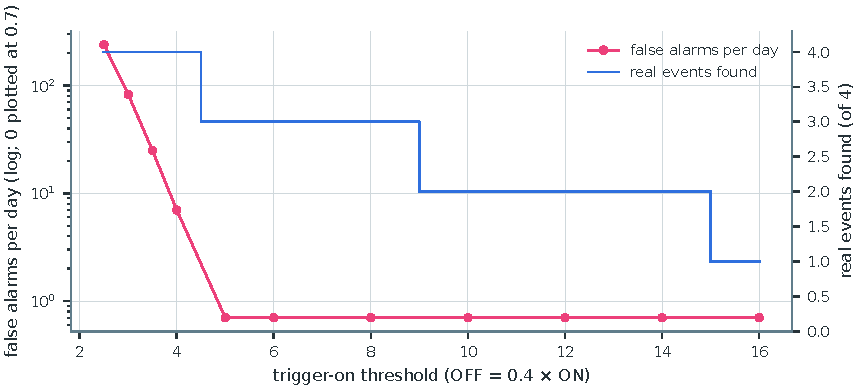
\includegraphics[width=\linewidth]{theory-stalta-sweep}
\caption{Sweep of the trigger-on threshold. False alarms (pink, left axis) vanish at 5; real events found (blue, right
axis) fall from 4 to 3 at that threshold, because the distant earthquake is lost, then to 2 and 1 as the two noise
bursts are lost one after the other; at the highest thresholds only the local earthquake remains.}\label{fig:sweep}
\end{figure}

\section{Failure modes and how to reduce them}\label{sec:failures}
\subsection{Man-made noise looks like an earthquake}
The two noise bursts of the demo day exceed the threshold by a wide margin: to an energy detector a person stamping next to
the sensor and a small local earthquake are both a sudden rise in power. \Cref{fig:compare} shows the difference that
can be exploited: the earthquake keeps a long, decaying \emph{coda} and the ratio stays elevated, whereas the
burst stops abruptly and the ratio collapses within seconds. Criteria that use this are a minimum duration, the ratio's
persistence, and the frequency content (the burst is broadband, the earthquake concentrated in 2--8~Hz).

\begin{figure}[tbp]
\centering
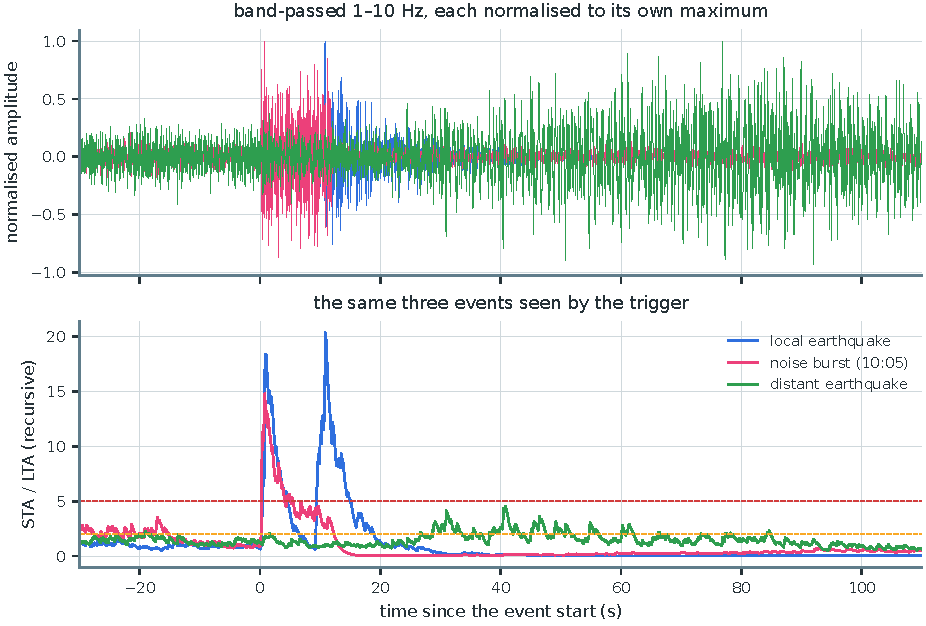
\includegraphics[width=\linewidth]{theory-stalta-compare}
\caption{Three events seen by the trigger, each aligned at its start. The earthquake (blue) keeps a decaying coda; the
burst (pink) stops after 12~s; the distant earthquake (green) never reaches the threshold because its energy lies
below the 1--10~Hz pass band.}\label{fig:compare}
\end{figure}

\subsection{Other failure modes}
\begin{description}[leftmargin=2.4cm,style=nextline]
\item[Gaps] a gap must reset the long average; otherwise the first samples after the gap are compared with a stale
  background. The detector treats each contiguous stretch separately and observes the warm-up period after each gap.
\item[Offset steps and spikes] a step in the DC level or a single instrument spike produces a short, large CF. The
  band-pass removes steps; a spike is removed by a minimum duration.
\item[LTA contamination] a long event raises the LTA and lowers the ratio for a while after it, so an aftershock may be
  missed. Some detectors \emph{freeze} the LTA while a trigger is active.
\item[Slow rise of noise] the LTA lags a steadily rising noise level, which keeps $R>1$; a rising wind can cause a
  false alarm.
\item[Weak distant events] emergent, long-period events lie outside a 1--10~Hz band; a detector for them needs a
  different band and longer windows (the sweep shows the distant earthquake lost already at $r=5$).
\end{description}

\section{Latency}\label{sec:latency}
How soon after an event begins does the trigger fire? Assume that the CF power jumps at $t=0$ from the background $P_0$ to
$P_1$ and that the LTA hardly changes in the first seconds. With the recursive STA of~\eqref{eq:rec}, whose time constant is
$\tau_s$,
\begin{equation}
  \mathrm{STA}(t) = P_1 + (P_0-P_1)\,e^{-t/\tau_s}.
\end{equation}
The ratio reaches $r_{\mathrm{on}}$ when $\mathrm{STA}=r_{\mathrm{on}}P_0$, at the delay
\begin{equation}\label{eq:delay}
  t_d = -\tau_s\,\ln\!\left(\frac{P_1-r_{\mathrm{on}}P_0}{P_1-P_0}\right),\qquad P_1>r_{\mathrm{on}}P_0 .
\end{equation}
Equation~\eqref{eq:delay} has two consequences. A strong event ($P_1\gg r_{\mathrm{on}}P_0$) triggers after a small fraction
of $\tau_s$: for a power increase of $100\times$ and $r_{\mathrm{on}}=5$, $t_d=0.04\,\tau_s$. A weak event
($P_1\to r_{\mathrm{on}}P_0$) takes arbitrarily long, and one with $P_1\le r_{\mathrm{on}}P_0$ is never detected at all.
(Appendix~\ref{app:delay} derives the formula.) The trigger time is therefore a \emph{detection} time, not an onset
time; for the onset the pass band must be causal and a dedicated picker must refine it.

\section{Design of the RS3D alert pipeline}\label{sec:alertdesign}
\begin{rs3dwarn}[Design proposal]
The following is the design that is planned for the first implementation. It will be revised when the feature is built.
\end{rs3dwarn}

\paragraph{Goals.} Detect events on the live stream without a browser open; tell the user through the channels they
enabled; keep a permanent record; and never fail silently.

\paragraph{Architecture.} The detector runs as a background service inside the application process, fed from the same
ring buffer as the Live page (Chapter~\ref{ch:realtime}), so it keeps running when no browser tab is open.
\Cref{fig:alertarch} shows the stages and \cref{fig:alertstate} the logic of one detector.

\begin{figure}[tbp]
\centering
\resizebox{\linewidth}{!}{\begin{tikzpicture}[node distance=5mm and 8mm]
  \node[box] (buf) {ring buffer\\[-1pt]{\scriptsize live samples}};
  \node[box,right=of buf] (pre) {pre-processing\\[-1pt]{\scriptsize causal band-pass}};
  \node[box,right=of pre] (det) {STA/LTA\\[-1pt]{\scriptsize recursive}};
  \node[boxblue,right=of det] (logic) {event logic\\[-1pt]{\scriptsize thresholds, hold-off}};
  \node[box,below=of logic,xshift=-18mm] (s1) {on-screen\\[-1pt]{\scriptsize banner, sound}};
  \node[box,right=of s1] (s2) {desktop\\[-1pt]{\scriptsize notification}};
  \node[box,right=of s2] (s3) {message\\[-1pt]{\scriptsize Telegram, e-mail}};
  \node[box,right=of s3] (s4) {record\\[-1pt]{\scriptsize plot and log}};
  \draw[flow] (buf) -- (pre); \draw[flow] (pre) -- (det); \draw[flow] (det) -- (logic);
  \foreach \s in {s1,s2,s3,s4} {\draw[flow] (logic.south) -- ++(0,-2mm) -| (\s.north);}
\end{tikzpicture}}
\caption{Proposed alert pipeline. Each output on the bottom row is an independent switch in Settings, and the record is
always written.}\label{fig:alertarch}
\end{figure}

\begin{figure}[tbp]
\centering
\begin{tikzpicture}[node distance=14mm,every node/.style={font=\small\sffamily}]
  \node[boxdark] (warm) {warm-up};
  \node[boxblue,right=18mm of warm] (idle) {idle};
  \node[box,right=24mm of idle,fill=rs3dred!15,draw=rs3dred] (act) {active};
  \node[box,right=18mm of act] (cool) {hold-off};
  \draw[flow] (warm) -- node[above]{$N_l$ samples} (idle);
  \draw[flow] (idle) -- node[above]{$R>r_{\mathrm{on}}$} (act);
  \draw[flow] (act) -- node[above]{$R<r_{\mathrm{off}}$} (cool);
  \draw[flow] (cool.south) -- ++(0,-8mm) -| node[pos=0.25,below]{quiet for hold-off} (idle.south);
  \draw[flow] (cool.north) -- ++(0,6mm) -| node[pos=0.25,above]{$R>r_{\mathrm{on}}$ again: same event} (act.north);
  \draw[flow,dashed] (idle.north) -- ++(0,9mm) -| node[pos=0.25,above]{gap: restart} (warm.north);
\end{tikzpicture}
\caption{State of one detector. A new crossing during the hold-off period extends the same event, which is how the two
trigger intervals of \cref{fig:stalta} become one event.}\label{fig:alertstate}
\end{figure}

\paragraph{Event record.} Each event stores the onset time, the duration, the peak STA/LTA ratio, the peak amplitude (in counts, and in
m/s if the response is cached), the dominant frequency, the channel(s), and a snapshot of the waveform with its helicorder
position. This is what the user sees in the notification and what the saved plot and log contain.

\paragraph{Proposed initial parameters.} They come from the demo-day analysis above and are meant as a starting point to be
tuned on real data from the user's site.

\begin{table}[tbp]
\centering\small
\caption{Proposed initial alert parameters (design proposal).}\label{tab:alertparams}
\begin{tabularx}{\linewidth}{@{}l c X@{}}
\toprule
Parameter & Initial value & Reason\\ \midrule
Channel & EHZ & the vertical channel carries the P wave cleanly\\
Band-pass & 1--10~Hz, causal 4th order & local events; matches the Live default\\
STA / LTA & 1~s / 30~s & \cref{fig:stalta,fig:params}\\
$r_{\mathrm{on}}$ / $r_{\mathrm{off}}$ & 5 / 2 & zero false alarms on the demo day (\cref{fig:sweep})\\
Hold-off & 30 s & merges the P and S trigger intervals\\
Minimum duration & 2 s & rejects single-sample spikes\\
Warm-up & $N_l/\fs$ and after every gap & the LTA is not valid before\\
\bottomrule
\end{tabularx}
\end{table}

\paragraph{Known limitation.} An energy trigger cannot tell an earthquake from a burst of equal power. The first release will
report both, label an event ``short, no coda'' when it ends within a few seconds, and leave the decision to the user. The
criteria of Section~\ref{sec:failures} are candidates for later versions.

\paragraph{Comparison with rsudp.} The widely used \emph{rsudp} software \parencite{rsudp} also raises alerts from an
STA/LTA ratio on a Raspberry Shake stream. Community examples use a 6~s STA and a 30~s LTA and thresholds between about 1 and
4, with the observation that suitable thresholds depend strongly on the filter band and on site noise; no authoritative list of
its built-in defaults could be located while this manual was written, so none is quoted here. RS3D's alerts are intended to
complement it, with the added record-keeping and the helicorder and detail views of the application.

\chapter{Real-time data handling}\label{ch:realtime}

The Live page and the future alert service both consume a continuous stream. This chapter describes how that stream is
received, buffered and kept alive, and how the other path, the download of day files, works.

\section{SeedLink}
SeedLink is a protocol for distributing seismic data over TCP. A client connects to the server (on a Shake, port~18000),
asks which stations and streams it offers (\code{INFO STREAMS}), selects the channels it wants, and then simply
receives miniSEED records as they are completed by the digitiser. The application uses ObsPy's
\code{EasySeedLinkClient} for the protocol.

\begin{rs3dapp}
\file{core/seedlink.py} first \emph{probes} the Shake (connect, parse the XML answer of \code{INFO STREAMS}, disconnect)
to learn the network, station, location and channel names, which is what the Status page and \ui{Find Shake} use. The
streaming class \code{SeedLinkSource} then selects \code{EHZ}, \code{EHN} and \code{EHE}. ObsPy reconnects by itself
inside its collect loop, but its defaults (120~s idle timeout, 30~s delay) are far too slow for a live display, so the
application lowers them to a 10~s network timeout and a 2~s delay. One workaround is documented in the source: the
client is created with \code{autoconnect=False} and connected manually, because ObsPy~1.5.1 crashes when a timeout is
set after an automatic connection.
\end{rs3dapp}

\section{The ring buffer}
Incoming records are appended to a \emph{ring buffer} that holds the most recent 10~minutes per channel. Records arrive
in short pieces (typically a few seconds each); the buffer stores each channel as a list of \emph{contiguous chunks}:
a new piece is appended to the last chunk when it continues it exactly (same sampling rate, start within half a
sample interval of the previous end) and otherwise starts a new chunk, so every chunk is gap-free by construction.
Chunks that end more than 600~s before the newest data are discarded. All access is guarded by a lock, because
the receiving thread writes while the display thread reads.

To draw, the display asks for a \emph{snapshot}: the samples of one channel in the window $[t_e-W,\,t_e]$, where $t_e$
is the newest time and $W$ the chosen window (30~s to 10~min). The snapshot is assembled from the chunks, with a
\code{NaN} separator between chunks so that gaps stay visible. If a band-pass is requested it is applied to each chunk on
its own (Chapter~\ref{ch:filter}); then, if more than 1500 points remain, min/max decimation (Chapter~\ref{ch:vis})
reduces them. The page redraws every 0.25~s, and \ui{Pause} freezes the picture while the buffer continues to fill.

\section{Keeping the link alive}
Networks fail: a cable is unplugged, a Shake restarts. The streaming thread therefore runs a small state machine
(\cref{fig:reconnect}). It starts in \emph{connecting}; when the first record arrives it is \emph{live}; when the
connection ends or fails it waits and tries again in \emph{reconnecting}. The wait grows with each consecutive failure along the
sequence
\begin{equation}
  \text{back-off} = 2,\ 4,\ 8,\ 16,\ 30\ \text{seconds}\quad(\text{then 30 s}),
\end{equation}
so a Shake that is off for an hour is not polled every two seconds, and the sequence restarts at 2~s as soon as a connection
has delivered data. A second condition covers the case where the TCP connection survives but data stop: if no record
has arrived for 5~seconds while the state is \emph{live}, the page shows \emph{waiting for data}. When a connection
error is the reason, the reason text (for example \emph{connection refused}) is shown next to \emph{reconnecting}.

\begin{figure}[tbp]
\centering
\begin{tikzpicture}[every node/.style={font=\small\sffamily}]
  \node[box] (stop) at (0,0) {stopped};
  \node[box] (conn) at (4.2,0) {connecting};
  \node[boxblue] (live) at (10.6,0) {live};
  \node[box,fill=rs3damber!20,draw=rs3damber] (rec) at (6.6,-2.3) {reconnecting};
  \draw[flow] (stop) -- node[above]{start} (conn);
  \draw[flow] (conn) -- node[above]{first record} (live);
  \draw[flow] (conn.south) -- ++(0,-0.6) |- node[pos=0.25,left]{error} (rec.west);
  \draw[flow] (live.south) -- ++(0,-0.6) |- node[pos=0.25,right]{link lost} (rec.east);
  \draw[flow] (rec.north) -- node[right,pos=0.5,align=left]{wait 2, 4, 8, 16, 30~s,\\then retry} (6.6,-0.9) -| (conn.south east);
  \draw[flow,dashed] (live.north west) to[out=110,in=70,looseness=7] node[above=1pt]{no data for 5~s: ``waiting''} (live.north east);
\end{tikzpicture}
\caption{States of the live connection. The back-off sequence resets when a connection has delivered data.}\label{fig:reconnect}
\end{figure}

\begin{rs3dapp}
\code{RingBuffer}, \code{LiveStream} and the constants \code{BACKOFF}$=(2,4,8,16,30)$ are in \file{core/live.py}; the
display loop is in \file{app/pages/live.py}. Data are not persisted by the live path: the Live page shows what the buffer
holds; permanent data come from the Shake's own archive through the Data page.
\end{rs3dapp}

\section{Downloading the archive}
The Shake writes its own SDS archive. The application copies day files with SFTP over the same SSH login that the Status
page uses. For each selected channel it lists the remote days, compares them with the days already on the laptop, and fetches
the missing ones \emph{plus the newest remote day}, which is still growing. A file is first written as
\file{<name>.part} and renamed when complete, so a transfer cut by a cable fault leaves no corrupt day file. Reading
is read-only on the Shake; the application never modifies it.

\section{Latency}
The delay between ground motion and the picture has three parts: the digitiser must complete a record before sending
it (a few seconds), the network adds milliseconds on a direct cable, and the page refreshes every 0.25~s. A practical
latency of a few seconds is therefore expected, and is set by the record length, not by the application's processing.

\chapter{Software architecture}\label{ch:arch}

This chapter describes how the code is organised, so that the algorithms of the preceding chapters can be found, tested
and changed.

\section{Two layers}
The package \code{rs3d} has two layers with a strict dependency direction.

\begin{figure}[tbp]
\centering
\begin{tikzpicture}[node distance=5mm]
  \node[boxblue,minimum width=0.9\linewidth] (app) {\textbf{app/} --- NiceGUI pages, ECharts option builders, strings, state\\
    {\small status, live, helicorder, data, settings, guide \textbullet\ charts \textbullet\ detail panel}};
  \node[box,minimum width=0.9\linewidth,below=of app] (core) {\textbf{core/} --- signal processing and data access; no user-interface imports\\
    {\small spectro, helicorder, health, coverage, export, live, store, archive, seedlink, response, status}};
  \node[boxdark,minimum width=0.9\linewidth,below=of core] (lib) {ObsPy \textbullet\ SciPy \textbullet\ NumPy \textbullet\ matplotlib \textbullet\ paramiko \textbullet\ keyring \textbullet\ psutil};
  \draw[flow] (app) -- (core);
  \draw[flow] (core) -- (lib);
\end{tikzpicture}
\caption{Layers of the application. Arrows point from a layer to the layer it uses.}\label{fig:layers}
\end{figure}

\begin{description}[leftmargin=2.2cm,style=nextline]
\item[\code{core/}] every algorithm in this manual. These modules know nothing of the browser; they take and return ObsPy
  streams, NumPy arrays and plain data classes, which makes them testable in milliseconds with synthetic signals.
\item[\code{app/}] presentation. The chart builders in \file{app/charts.py} are \emph{pure functions} that return the
  option dictionaries of the charting library, so even the shape of a plot is unit-tested without a browser.
\end{description}

\section{Where each algorithm lives}
\Cref{tab:modules} maps every topic of this manual to the module and the main functions that implement it.
\begin{table}[tbp]
\centering\footnotesize
\caption{Algorithm $\to$ module.}\label{tab:modules}
\begin{tabular}{@{}L{0.20\linewidth}L{0.25\linewidth}L{0.40\linewidth}@{}}
\toprule
Topic & Module & Main functions\\ \midrule
Day-file layout, import & \file{core/store.py} & \code{day\_path}, \code{load}, \code{import\_file}\\
Response, units, filtering & \file{core/response.py}, \file{export.py} & \code{get\_inventory}, \code{process}\\
Spectra, spectrogram, noise & \file{core/spectro.py} & \code{amplitude\_spectrum}, \code{spectrogram}, \code{window\_for}, \code{psd\_summary}\\
Completeness, coverage & \file{core/health.py}, \file{coverage.py} & \code{health}, \code{coverage}\\
Helicorder rows and windows & \file{core/helicorder.py} & \code{build\_rows}, \code{scale\_for}, \code{click\_to\_time}, \code{zoom\_window}, \code{box\_window}\\
Decimation, live buffer & \file{core/live.py} & \code{minmax\_decimate}, \code{RingBuffer}, \code{LiveStream}\\
Shake access & \file{core/seedlink.py}, \file{shell.py}, \file{archive.py} & \code{probe}, \code{SeedLinkSource}, \code{sync}\\
Plot shapes & \file{app/charts.py} & \code{helicorder\_options}, \code{spectrogram\_options}, \code{psd\_options}\\
Detail view, clipboard & \file{app/detail.py}, \file{core/export.py} & \code{DetailPanel}, \code{write\_clipboard\_png}\\
\bottomrule
\end{tabular}
\end{table}

\section{Reproducibility by construction}
The Data page can show, and save, a short Python program that reproduces exactly the processing behind a preview: it
reads the same day files, applies the same response removal and the same band-pass, and prints the stream. The program is
generated by \file{core/codegen.py} from the same \code{Selection} object that the application itself uses, so the code
and the screen cannot drift apart. A researcher can therefore take any number off the screen and recompute it outside the
application.

\section{Testing}
Three levels of test protect the algorithms.
\begin{enumerate}
\item \textbf{Unit tests} of \file{core/} with synthetic data: a sine must peak in its own bin and read its own amplitude, a
  spike must survive decimation, a gap must stay a gap, a click must map to its row and time.
\item \textbf{Page tests} with NiceGUI's user simulation: each page renders with a fake device; controls change state as
  expected.
\item \textbf{Real-browser tests} (Playwright with Google Chrome, marker \code{e2e}): import a file, open the helicorder, click
  a row, zoom with a dragged rectangle, open the clipboard and download the picture. Each such test has been shown to fail when
  the behaviour it protects is deliberately broken.
\end{enumerate}
A fourth marker, \code{device}, selects tests that need a real Shake and is skipped by default.

\section{Configuration and storage}
All files live in one folder (on Linux \file{\textasciitilde/.local/share/rs3d}, overridable with the
\code{RS3D\_DATA\_DIR} environment variable): \file{config.toml} (devices), \file{settings.toml} (time zone, last station,
units and band-pass), \file{known\_hosts}, \file{sds/} (data), \file{response/} (StationXML cache), \file{logs/}. Passwords
are kept in the operating system's key store through \code{keyring}, never in these files.

\appendix
\chapter{Derivations}\label{app:deriv}

\section{Scaling of the amplitude spectrum}\label{app:scale}
Let $x[n]=A\cos(\theta n)$ with $\theta=2\pi f_0/\fs$, and let the window be $w[n]$, $n=0,\dots,N-1$. Write
$x[n]=\tfrac A2\bigl(e^{\jj\theta n}+e^{-\jj\theta n}\bigr)$. The windowed DFT at a bin with $2\pi k/N=\theta$ is
\begin{align}
  X_w[k] &= \sum_{n}w[n]\,x[n]\,e^{-\jj\theta n}
  = \frac A2\sum_{n}w[n]\;+\;\frac A2\sum_{n}w[n]\,e^{-\jj2\theta n}.
\end{align}
The second sum is the window's transform at twice the tone frequency, far outside the main lobe, and is negligible for a
tapered window. Hence $\abs{X_w[k]}\approx\tfrac A2\sum_nw[n]$, which is Eq.~\eqref{eq:ampscale}. If only a subset
$\mathcal V$ of the samples is valid and the others are set to zero, the first sum runs over $\mathcal V$ and the scale becomes
$\sum_{n\in\mathcal V}w[n]$, the rule used by the application.

\section{Hann window constants}\label{app:hann}
For $w[n]=\tfrac12\bigl(1-\cos\frac{2\pi n}{N-1}\bigr)$ and large $N$, the mean over a full period of the cosine is zero, so
$\sum w\approx N/2$, giving a coherent gain of $\tfrac12$. For the energy, with $c=\cos\frac{2\pi n}{N-1}$ averaging to 0 and $c^2$ to $\tfrac12$,
\[
  \sum w^2\approx N\,\overline{\tfrac14\bigl(1-2c+c^{2}\bigr)}=\tfrac N4\bigl(1+\tfrac12\bigr)=\tfrac{3N}{8}.
\]
The equivalent noise bandwidth is therefore
\[
  \mathrm{ENBW}=\frac{N\sum w^2}{(\sum w)^2}=\frac{N\cdot 3N/8}{N^2/4}=1.5\ \text{bins},
\]
matching Table~\ref{tab:windows}.

\section{Zero-phase filtering}\label{app:zp}
Let a filter have impulse response $h$ and frequency response $H(\omega)$. Filtering forward gives $Y_1=H X$. Time reversal of a real
sequence turns its transform into the complex conjugate (up to a linear phase that is undone by the second reversal), so the
backward pass multiplies by $H^{*}$ and the final reversal restores the time direction: $Y=H^{*}H\,X=\abs{H}^{2}X$. The
magnitude response in decibels is $20\log_{10}\abs{H}^{2}=2\cdot20\log_{10}\abs{H}$, twice that of one pass, so the $-3$~dB corner of one
pass is a $-6$~dB corner of the zero-phase filter.

\section{The recursive averages}\label{app:rec}
Rearranging Eq.~\eqref{eq:rec}: $\mathrm{STA}_i=(1-\tfrac1N)\mathrm{STA}_{i-1}+\tfrac1N c[i]$. Unrolling,
\begin{equation}
  \mathrm{STA}_i = \frac1N\sum_{k=0}^{i}\Bigl(1-\frac1N\Bigr)^{k}c[i-k]+\Bigl(1-\frac1N\Bigr)^{i+1}\mathrm{STA}_{-1}.
\end{equation}
The weights sum to $1-(1-1/N)^{i+1}\to1$ and, for large $N$, $(1-1/N)^{k}\approx e^{-k/N}$: an exponential window of time
constant $N$ samples. The initial-condition term decays with the same time constant, which is why a warm-up of $N_l$ samples is
needed.

\section{Detection delay}\label{app:delay}
For a step of the CF power from $P_0$ to $P_1$ at $t=0$ the continuous-time analogue of~\eqref{eq:rec} is
$\dot{S}=(P_1-S)/\tau_s$ with $S(0)=P_0$, whose solution is $S(t)=P_1+(P_0-P_1)e^{-t/\tau_s}$. Setting
$S(t_d)=r_{\mathrm{on}}P_0$ and solving for $t_d$,
\[
  e^{-t_d/\tau_s}=\frac{P_1-r_{\mathrm{on}}P_0}{P_1-P_0}
  \;\Rightarrow\;
  t_d=-\tau_s\ln\frac{P_1-r_{\mathrm{on}}P_0}{P_1-P_0},
\]
which is Eq.~\eqref{eq:delay}. The assumption that the LTA is constant during $t_d$ holds when $t_d\ll\tau_l$; for $\tau_l=30$~s and
$\tau_s=1$~s it is good for all events strong enough to trigger within a few seconds.

\section{The $F$ distribution of the ratio}\label{app:f}
If the CF is the square of zero-mean Gaussian noise of variance $\sigma^{2}$ filtered to bandwidth $B$, the average of $c$ over $T$ seconds is
$\sigma^{2}\chi^{2}_{\nu}/\nu$ with $\nu\approx2BT$ degrees of freedom (the number of independent samples is about $2BT$, by the
sampling theorem). The STA and LTA are independent only if their windows do not overlap, which the classic form approximately
satisfies, and then $R=\dfrac{\chi^{2}_{\nu_s}/\nu_s}{\chi^{2}_{\nu_l}/\nu_l}\sim F_{\nu_s,\nu_l}$. The tail probabilities of
Table~\ref{tab:null} are $1-F_{\nu_s,\nu_l}(r)$ with $\nu_s=18$, $\nu_l=540$. They apply to \emph{one} independent evaluation;
the number of false alarms per day also depends on how many independent evaluations occur and on how exceedances cluster,
which is why the table reports simulated counts alongside the tail.

\section{Error of min/max decimation}\label{app:mm}
Let a bin contain samples $x[n]$, $n\in b$, and let $\hat x$ denote the drawn polyline through the kept extremes. Every sample of the bin lies
between its minimum and maximum, so the vertical distance between any sample and the plotted bin is at most
$x^{\max}_b-x^{\min}_b$, and the horizontal position of the extremes is exact. Therefore the plotted envelope
\[
  \bigl[\,x^{\min}_b,\ x^{\max}_b\,\bigr]
\]
equals the true envelope of the bin, and the only information lost is the order of the samples between the extremes.

\chapter{Parameter reference}\label{app:params}

Every numerical constant that shapes a result, with the file in which it is set (relative to \file{rs3d-app/src/rs3d/}).
\Cref{tab:paramA} covers acquisition and conditioning, \cref{tab:paramB} analysis and display, and \cref{tab:paramC}
the health checks.

\begin{table}[tbp]
\centering\small
\caption{Acquisition, buffering and conditioning.}\label{tab:paramA}
\begin{tabular}{@{}L{0.40\linewidth}L{0.27\linewidth}L{0.25\linewidth}@{}}
\toprule
Quantity & Value & File\\ \midrule
Sampling rate (RS3D) & 100~Hz & device\\
SeedLink port & 18000 & \file{core/models.py}\\
SeedLink network timeout / delay & 10~s / 2~s & \file{core/seedlink.py}\\
Ring buffer length & 600~s & \file{core/live.py}\\
Reconnect back-off & 2, 4, 8, 16, 30~s & \file{core/live.py}\\
Stale-data warning & 5~s & \file{core/live.py}\\
Live refresh interval & 0.25~s & \file{app/pages/live.py}\\
Live windows & 30, 60, 300, 600~s & \file{app/pages/live.py}\\
Live decimation limit & 1500 points & \file{app/pages/live.py}\\
Live band-pass default / order & 1--10~Hz / 2 (padded forward--backward) & \file{app/pages/live.py}, \file{core/live.py}\\
Live upper-corner limit & $0.45\,\fs$ & \file{core/live.py}\\
Export band-pass & Butterworth order 4, two passes, demeaned & \file{core/export.py}\\
Response removal & ObsPy defaults: water level 60~dB, 5\,\% taper & \file{core/export.py}\\
\bottomrule
\end{tabular}
\end{table}

\begin{table}[tbp]
\centering\small
\caption{Spectral analysis, helicorder and detail view.}\label{tab:paramB}
\begin{tabular}{@{}L{0.40\linewidth}L{0.27\linewidth}L{0.25\linewidth}@{}}
\toprule
Quantity & Value & File\\ \midrule
Amplitude-spectrum window & Hann, scale $2/\sum w$ & \file{core/spectro.py}\\
Minimum samples for a spectrum & 8 & \file{core/spectro.py}\\
Spectrogram window & SciPy default Tukey ($\alpha=0.25$) & \file{core/spectro.py}\\
Spectrogram overlap & 50\,\% & \file{core/spectro.py}\\
Window-length rule & $T/360$, limited to 1--600~s & \file{core/spectro.py}\\
Noise-spectrum percentiles & 10, 50, 90 & \file{core/spectro.py}\\
Spectrogram heat-map size & at most $400\times200$ cells & \file{app/charts.py}\\
Spectrogram colour range & 2nd--98th percentile & \file{app/charts.py}\\
Data-page waveform thinning & stride to about 4000 points & \file{app/charts.py}\\
Helicorder row length / rows & 30~min / 48 & \file{core/helicorder.py}\\
Points per helicorder row & 3000 & \file{core/helicorder.py}\\
Helicorder amplitude scale & $2P_{99}/F$, $F\in\{0.5,1,2,4,8\}$ & \file{core/helicorder.py}\\
Helicorder row height / click grid & 14~px / every 10~s & \file{app/charts.py}\\
Detail window, default & 120~s & \file{app/detail.py}\\
Detail window limits & 5~s -- 3600~s & \file{core/helicorder.py}\\
Zoom factors / shift & $\times2$, $\times\tfrac12$ / $\pm\tfrac12$ span & \file{core/helicorder.py}\\
Box-zoom amplitude rounding & 4 significant figures & \file{app/detail.py}\\
\bottomrule
\end{tabular}
\end{table}

\begin{table}[tbp]
\centering\small
\caption{Data health and Shake checks.}\label{tab:paramC}
\begin{tabular}{@{}L{0.40\linewidth}L{0.27\linewidth}L{0.25\linewidth}@{}}
\toprule
Quantity & Value & File\\ \midrule
Gap merge tolerance (coverage, health) & $0.5/\fs$ & \file{core/coverage.py}, \file{core/health.py}\\
Helicorder gap break & $1.5/\fs$ & \file{core/helicorder.py}\\
Gaps listed on the Data page & at most 50 & \file{app/pages/data.py}\\
Clock offset: warning / error & $>100$~ms / $>1000$~ms & \file{core/status.py}\\
Free storage warning & $<10\,\%$ & \file{core/status.py}\\
Link-local address range & 169.254.0.0/16 & \file{core/netcheck.py}\\
Archive: day at risk & not downloaded and within one day of the retention limit & \file{core/status.py}\\
\bottomrule
\end{tabular}
\end{table}

\backmatter
\printbibliography[heading=bibintoc,title={References}]
\end{document}
